\documentclass[english]{htldipl}
% Zulässige Class Options: 
%   Hauptsprache: german (default), english

% die folgende Zeile einkommentieren für Arial-Ähnliche Schriftart
%\renewcommand{\familydefault}{\sfdefault}

\graphicspath{{images/}}    % wo liegen die Bilder?
%\usepackage[margin=3cm]{geometry} % alle Seitenränder auf 3 cm einstellen
\usepackage{makeidx}\makeindex
\usepackage[toc]{glossaries}\makeglossaries
\usepackage[parfill]{parskip}

\newglossaryentry{Fast Fourier Transformation}{
	name=Fast Fourier Transformation,
	description={
		A fast divide and conquer algorithm to transform signals from time domain into frequency domain. This is used to to get a frequency spectrum of an audio input}
}
\newacronym{FFT}{FFT}{Fast Fourier Transformation}

\newglossaryentry{MIDI}{
	name=MIDI,
	description={
		A protocol to describe timed events, in this case music notes}
}

\newglossaryentry{pick-up}{
	name=pick-up,
	description={
		A device that is used to record guitars. It is placed directly below the strings and many guitars have it already built-in}
}


%\glsaddall 
% commented out to avoid page 1 references

%%%----------------------------------------------------------
\begin{document}
%%%----------------------------------------------------------

\newcommand{\cpp}{\texttt{C++}\space}
\title{Beat the Score}
\abteilung{Informatik}
\schwerpunkt{}
\studienort{Wiener Neustadt}
\schule{HTBLuVA Wiener Neustadt}
\schullogo{htl.png}
\abgabejahr{2013/14}
\betreuerA{Dipl.-Ing. Dr. Günter Kolousek}
\betreuerB{}
\betreuerC{}
\betreuerD{}
\betreuerE{}
%\betreuerE{} oder leer lassen wenn nicht vorhanden
\schuelerA{Felix Kugler}
\evidenzA{5BHIF-10}
\schuelerB{Alfred Neumayer}
\evidenzB{5BHIF-13}
\schuelerC{Daniel Novotny}
\evidenzC{5BHIF-14}
\schuelerD{}
\evidenzD{}
\schuelerE{}
\evidenzE{}
\schuelerF{}
\evidenzF{}
\schuelerG{}
\evidenzG{}
%\schuelerG{} oder leer lassen wenn nicht vorhanden
%\evidenzG{} oder leer lassen wenn nicht vorhanden

%%%----------------------------------------------------------
\frontmatter
\maketitle
\tableofcontents
%%%----------------------------------------------------------


\chapter{Kurzfassung}

\emph{Beat the Score} ist ein Trainingsprogramm für beginnende Musiker. Es hilft dem Benutzer beim Üben die richtigen Noten zum richtigen Zeitpunkt zu treffen. Es erfolgt eine sofortige Rückmeldung darüber wie der Benutzer gespielt hat. Der Computer begleitet den Spieler dabei mit weiteren Instrumenten.

Durch Unterstützung des populären GP5 Formats kann der Benutzer eine große Auswahl an Noten im Internet finden.
Für Rückmeldung der Spielweise können Instrumente per Klinke oder USB an den Computer angeschlossen werden. Unterstützt werden Gitarren und Klaviere.

Da Anfänger oft nicht Notenschrift lesen können, werden verschiedene Anzeigemethoden angeboten: 
\begin{description}
	\item[Klaviatur] \hfil \\ Die Noten werden als Rechtecke angezeigt, wobei eine Achse die Tonhöhe und die andere den Zeitpunkt darstellt.
	\item[Notenschrift] \hfil \\ Wie sie unter Musikern üblich ist.
	\item[Tabulatur] \hfil \\ Wie sie von Gitarristen verwendet wird.
\end{description}

Zum Üben ist es auch möglich, das Tempo des Liedes einzustellen oder den Trainingsmodus zu aktivieren, wo bei jeder Note pausiert wird, bis die richtige Note gespielt wurde.

Das Programm ist erhältlich im Google Play Store für Android und auf der Website {\tt http://beatthescore.at} für Linux, Windows und in Zukunft auch Mac OSX.		
\chapter{Abstract}

\emph{Beat the Score} is a trainings program for amateur musicians. It helps to practice hitting the right notes at the right time by displaying notes for the user to play. It gives instant feedback about the note played and whether they were on time. Additional instruments are played by the computer.

By supporting the popular Guitar Pro 5 (GP5) format, the user can find a wide variety of songs available on the internet. 

To read what notes the user has played, they can connect their instrument via phone connector or USB. Supported are guitars and keyboards.

Since not everybody can read sheet music, three different display methods are supported: 
\begin{description}
	\item[Piano roll] \hfil \\ Notes are displayed as rectangles with the pitch being encoded in one axis and the time in the other.
	\item[Score] \hfil \\ Common sheet music.
	\item[Tablature] \hfil \\ As it is used by guitarists.
\end{description}

For training purposes we provide a trainings mode where the game pauses for every note and continues when the player plays the right keys. It is also possible to lower (or even increase) the tempo of a song. 

The program can be bought on the Google Play Store for Android tablets and on {\tt http://beatthescore.at} for Linux and Windows.			

%%%----------------------------------------------------------
\mainmatter           %Hauptteil (ab hier arab. Seitenzahlen)
%%%----------------------------------------------------------

\chapter[User Interaction Concept \textsuperscript{Novotny}]{User Interaction Concept}
 \label{chap:UserInteractionConcept}
\section{Menu Navigation}
The menu structure of the application is divided into four main parts. \\
\begin {itemize}
	\item {Main Menu}
	\item {Game Start Menu}
	\item {Options Dialog}
	\item {In-Game Menus}
\end {itemize}
The user interaction conecpt has been tailored to provide a comfortable user experience on desktop and mobile environments.
The layout of the menus has been designed to support an efficient navigation process. 

\subsection{Multidimensional User Interaction}
In order to provide an enjoyable user experience for both novices and experienced users, multiple ways of interacting with the user interface have been implemented.
\begin {itemize}
	\item {Mouse- and Touch-Based Navigation}
	\item {Keyboard-Based Navigation}
	\item {Sound-Based Navigation}
\end {itemize}
\paragraph{Keyboard-Based Navigation}
All parts of the user interface can be controlled using the keyboard exclusively. 

The following keys are used:

\begin{tabular}{ |l|l| }
  \hline
  \multicolumn{2}{|c|}{Key Map} \\
  \hline
  Arrow Keys (left / right) & pre-select item within focused list \\
  Arrow Keys (up / down) & select next / previous item in focus chain \\
  Tab / Back Tab & select next / previous item in focus chain \\
  Enter & confirm all selections and proceed (e.g. start game) \\
  Space & select pre-selected item \\
  ESC, Backspace & go back to previous menu \\
  \hline
\end{tabular}
\paragraph{Sound-Based Navigation}
All components of the application relevant to the user during a practice session can be controlled using the user´s instrument. \\
As the user might not have selected his desired input device by the time he switches to Sound-Based Navigation, notes played on any of the available devices is considered for this purpose.
Chords that the user plays on his instrument are recognized and mapped to functions of the user interface. Where applicable, the chords and their mapped functions are displayed on the user interface.\\
In order to make these functions easier to remember, certain types of chords are mapped to specific types of functionalities.
\begin {itemize}
	\item {Major chords cause a positive shift of focus or selection.}
	\item {Minor chords cause a negative shift of focus or selection.}
	\item {Diminished chords provide additional assistance to the user (e.g. displaying on-screen instructions)}
\end {itemize}
The chord \textbf{C Major} is globally reserved for confirming all settings of the current dialog and proceeding to the next step.\\
The chord \textbf{C Minor} is globally reserved for discarding all settings of the current dialog and going back to the last menu page. \\
\paragraph{Linear Navigation}
Linear navigation is used to guide a user to go from one step to another in a particular order. 
The idea behind linear navigation is that the user makes his selections in a predefined order or sequence. \\
The benefits of linear navigation include
\begin {itemize}
	\item { reducing the risk of the user omitting necessary information,}
	\item { making the process transparent and understandable for less experienced users,}
	\item { allowing keyboard- and soundbased navigation for experienced users.}
\end {itemize}
The concept of linear navigation has been implemented throughout the whole user interface. \\
The user can proceed to the next step by
\begin {itemize}
	\item {pressing associated keys on the keyboard (tab, arrows, ...),}
	\item {playing associated chords on one of the connected instrument.}
\end {itemize}.
\subsection{Main Menu} 
The Main Menu will be presented to the user as soon as the application has been initialized. 
It provides links to the Game Start Menu and the Option Menu.

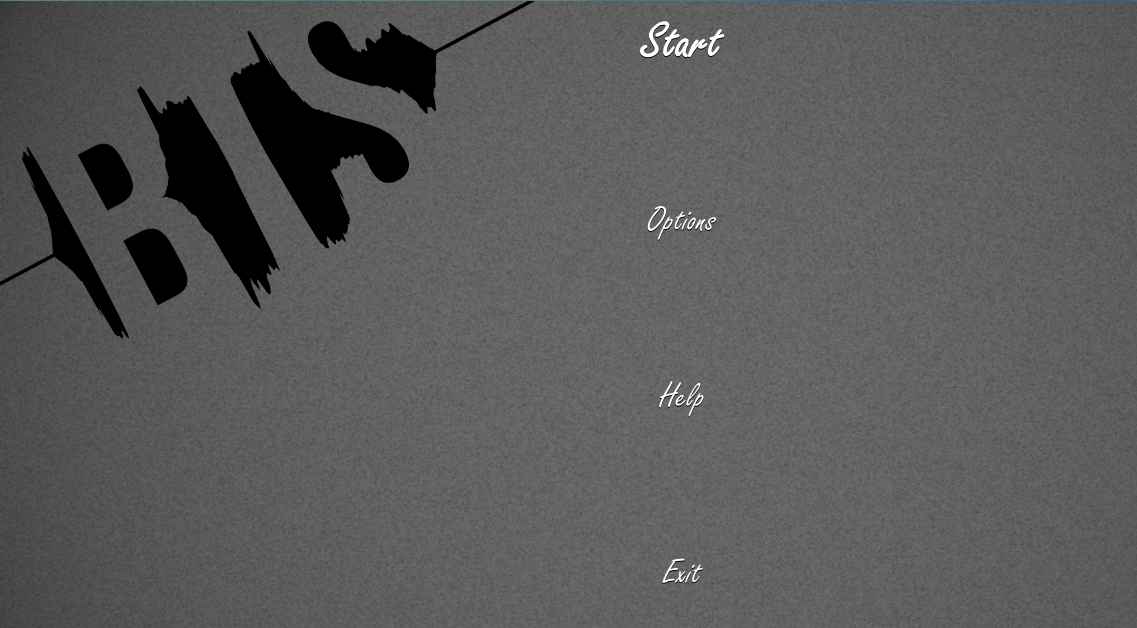
\includegraphics[width=\textwidth]{main_menu_2}

Returning to the main menu is possible from every point of the user interface.
In most cases, the user will use this menu to get to the Game Start Menu. Therefore, the corresponding item is preselected in order to enable fast keyboard- or sound-based selection.
\subsection{Game Start Menu}
The purpose of the Game Start Menu is to define the game situation the user would like to use. It is used right before the game is started which is expected to happen multiple times within a session.

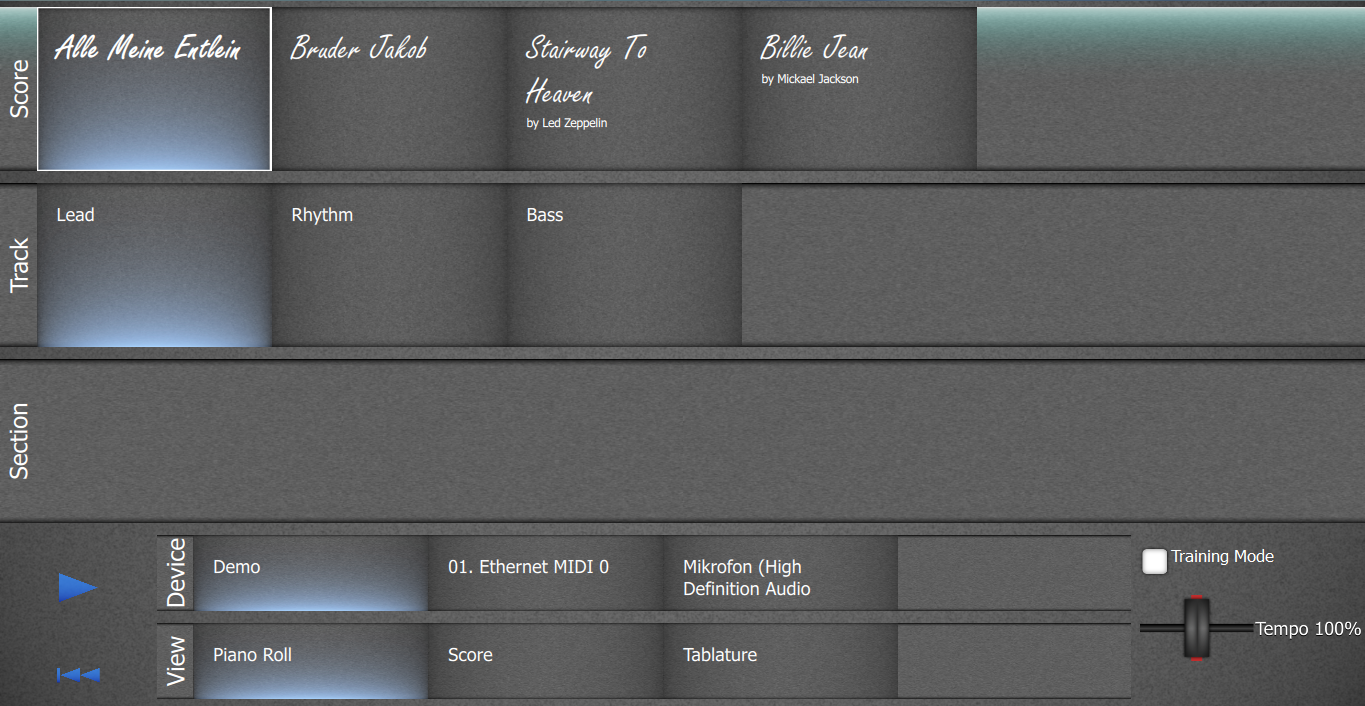
\includegraphics[width=\textwidth]{game_start_menu_2}
\paragraph{Main Flow}
The majority of user interactions inside the Game Start Menu consist of the following steps.
\begin {enumerate}
	\item {select the song, possibly using the search function to navigate through a wide selection of scores}
	\item {select the instrumental track withing the song}
	\item {select the section of the song to be practiced}
	\item {start the game}
\end {enumerate}
\paragraph{Preference Settings}
The following settings are expected to be changed on a less frequent basis:
\begin {itemize}
	\item {whether or not to use the training mode}
	\item {display option}
	\item {input device}
\end {itemize}
The menu layout is designed to make the main flow efficient and comfortable and to reduce the amount of necessary adjustments to the Preference Settings. \\
Linear navigation will guide the user through the items of the main flow, allowing corrections of previous selections while avoiding the need to skip settings that are rarely changed. The preference settings chain directly follows the main flow chain allowing smooth transitions between these sections. \\
The Preference Settings will be kept throughout the whole session. 
\paragraph{Search Function}
The application is designed to handle a wide selection of score files. In order to help the user to find the desired file quickly a search function has been implemented. 
\subsubsection{Focus, Pre-Selection and Selection}
The use of keyboard- and soundbased linear navigation requires the user to be aware which elements of the user interface are focused, pre-selected and selected at a certain time. Different types of highlighting are used to indicate the states of the elements.
\paragraph{Selection Process}
As mentioned earlier, the user interface supports keyboard and sound-based navigation. It allows both vertical and horizontal selection shifts. At multiple spots in the user interface, more than one component is placed in a row. Suppose a button and a horizontally aligned {\tt ListView} are placed in the same row. The horizontal arrows keys can be used to select an item within the {\tt ListView}. The user might however expect to be able to use these horizontal arrows keys to move to the other component placed on the left hand side or the right hand side of the {\tt ListView}.The example below demonstrates this issue. 

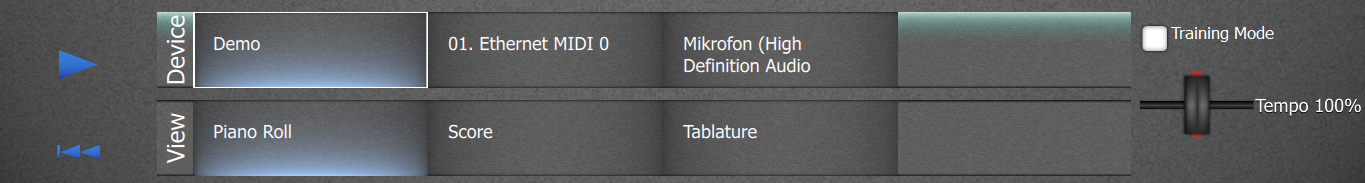
\includegraphics[width=\textwidth]{selection_issue_2}

In order to comply with user expectations two different stages of selection have been introduced:
\begin {itemize}
	\item {Pre-Selection}
	\item {Selection}
\end {itemize}
\paragraph{Pre-Selection}
Only items that are pre-selected can be selected using linear navigation. Pre-Selection can be moved using the horizontal arrows keys without changig the actual selection. This allows using the horizontal arrow keys when moving from one component within a row to another. Pre-Selected items are surrounded by a white border. 
\paragraph{Selection}
Pressing the Space key while a {\tt ListView} is focused will cause the pre-selected item to be selected. A highlight effect is used to indicate which item is currently selected.

In the example below the \textit{Rhythm} track of a song is selected. The \textit{Drum} track is preselected.

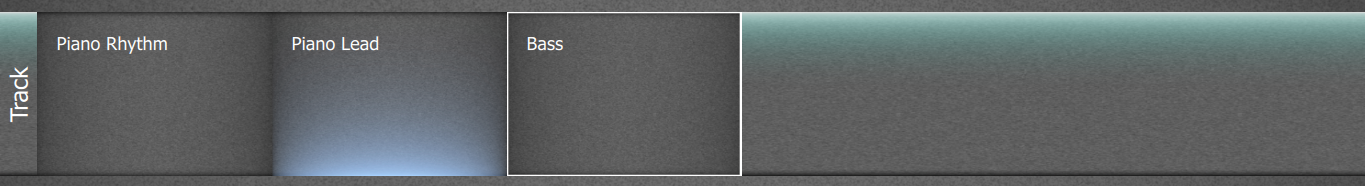
\includegraphics[width=\textwidth]{selection_process_2}
\subsection{Options Menu}
The Options Menu contains settings that affect the applications behaviour and are not directly relevant to the current session. 

Currently the options menu offers the following settings:
\begin{itemize}
	  \item{
		 whether or not preferences to keep preference settings for the next session
	  }
	  \item{
	  	whether or not audio inputs are offered as available devices in the game settings menu
	  }
	  \item{
	  	sampling rate for audio analysis
	  }
	  \item{
	  	default sound volume
	  }
\end{itemize}

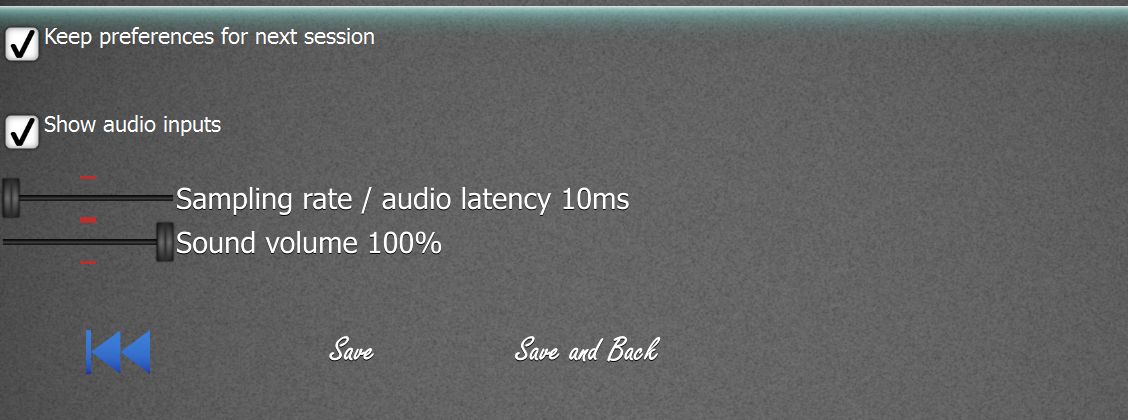
\includegraphics[width=\textwidth]{options_menu_2}

Linear navigation has been implemented similarly to the game settings menu. Sound-Based navigation has not been implemented because the settings in this section are not expected to be changed during the vast majority of sessions. 

\subsection{Pause Menu}
The game can be paused at any time.\\
The pause menu has the following features:
\begin {itemize}
	\item {Adjusting the volume of the audio output}
	\item {Returning to the Game Start Menu}
\end {itemize}

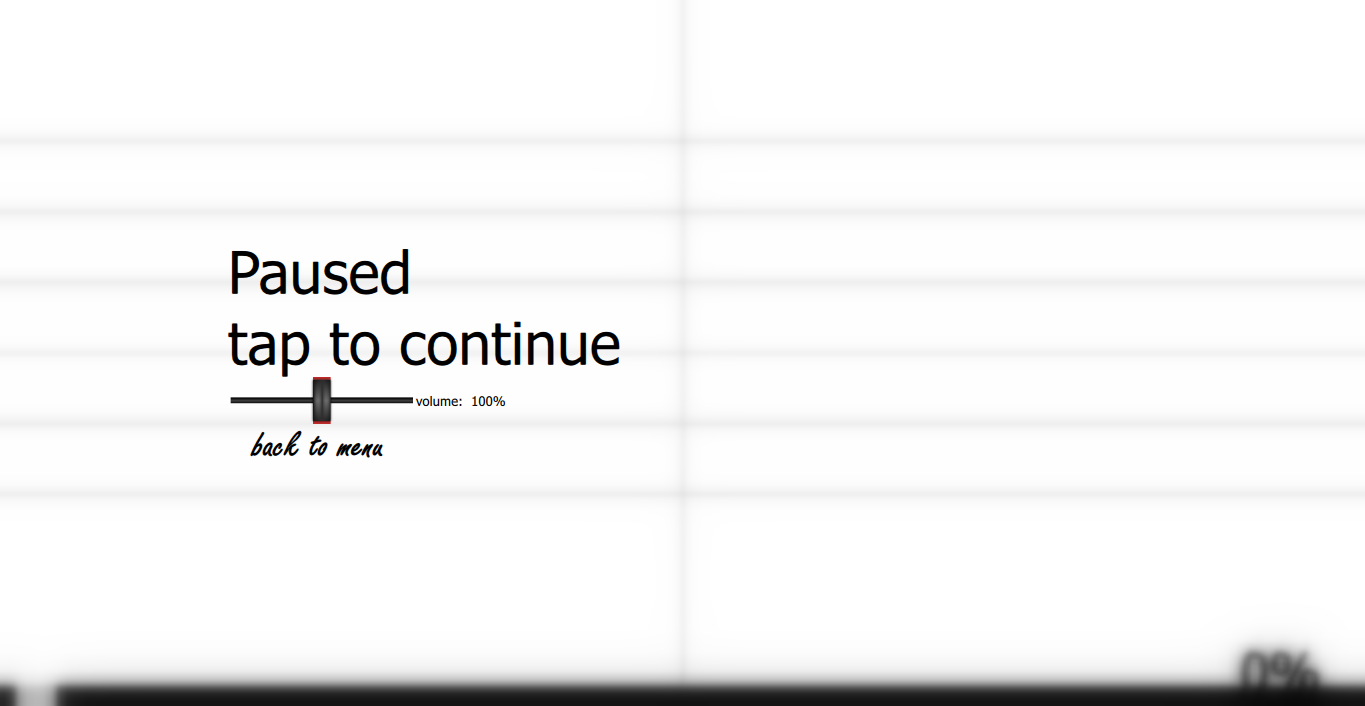
\includegraphics[width=\textwidth]{pause_menu}

Sound navigation has not been implemented for the Pause Menu because a chord associated with calling the Pause Menu might coincide with notes contained in the song.

\subsection{Result Screen}
The Result Screen appears once a song has finished.

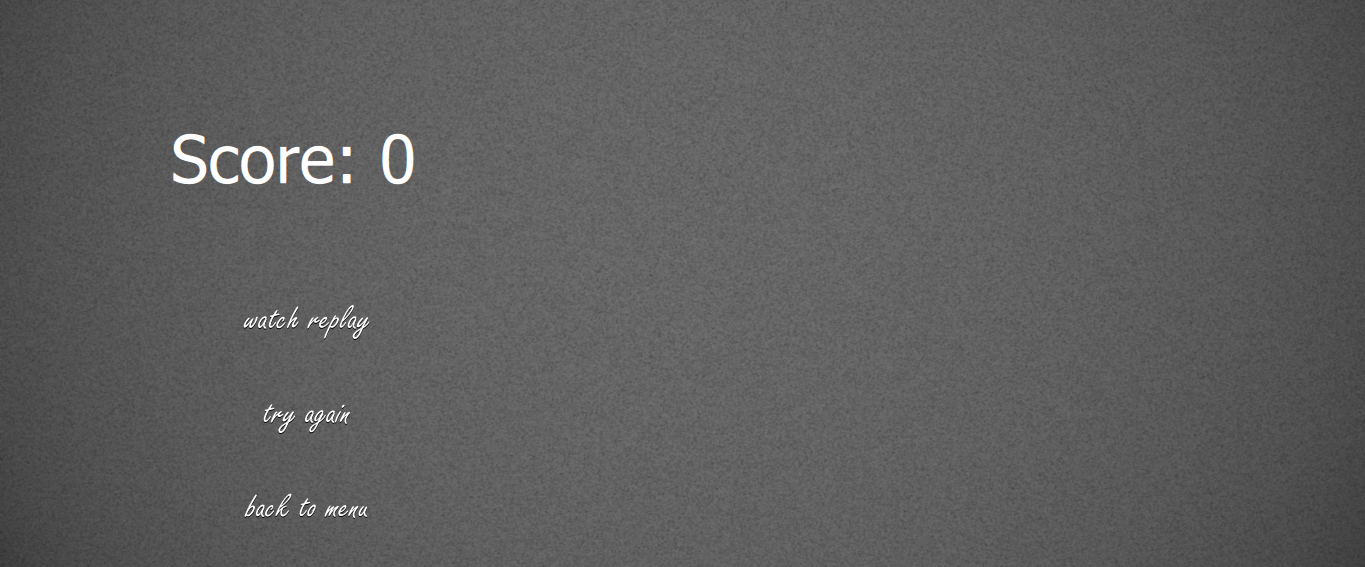
\includegraphics[width=\textwidth]{result_screen_2}

It has the following functions:
\begin {itemize}
	\item{Displaying the score the user has achieved}
	\item{Allowing the user to decide what to do next} 
\end {itemize}
Once the song has finished, the user has the following options on how to proceed:
\begin {itemize}
	\item {Watch a replay of his performance}
	\item {Try to play the same song again}
	\item {Go back to the Game Settings Menu}
\end {itemize}
\chapter[Basic Musical Terms and Concepts \textsuperscript{Novotny}]{Basic Musical Terms and Concepts}
\label{chap:Basic Musical Terms}

\paragraph{Organisation of the Chapter}
This chapter explains basic terms and concepts related to music, music theory, and musical instruments that will be used throughout the following chapters. Note that the treatment of the concepts in this chapter is very brief and informal. It is inteded to give the layman an overview of the topic that is sufficient for understanding the following chapters.

\section{Musical Terms}
\paragraph{Note}
\index{Note}
Primarily a note consits of:

\begin{itemize}
	\item{pitch}
	\item{duration}
\end{itemize}

In the context of this project a note contains the following additional information:
\begin{itemize}
	\item{position within the score (see \ref{sec:score})}
	\item{where on the fretboard the note is played (relevant for string instruments)}
	\item{the way the note is played (in terms of playing techniques)}
\end{itemize}

\paragraph{Chord}
\index{Chord}
\index{Triad}
A chord is a set of at least three notes played at the same time. 
The term \textit{Triad} refers to a chord that consists of exactly three notes. Triads are the only types of chords relevant to the project. This does not mean that chords of more than three notes contained in scores can not be displayed, recognised and played properly, refer to later chapters for clarification.

There are four types of triads, commonly referred to as chord qualities:
\begin{itemize}
	\item{major}
	\item{minor}
	\item{augmented}
	\item{diminished}
\end{itemize}

A chord is typically referred to by its root note and its quality (for example \textit{D Major, E Minor}).

A chord is called \textit{inverted} if the lowest note of the chord is not the root note. A \textit{C Major} chord consists of the notes \textit{C, E, G}. If a \textit{C} chord is rearranged in a way such that \textit{E} is the lowest note of the chord this \textit{inversion} of the chord is commonly referred to as a \textit{C/E} chord.

\paragraph{Score}
\label{sec:score}
Scores are analog, visual representations of musical pieces. A score consists of notes and are notated in one of the forms of musical notations discussed in the next section.

\section{Musical Notation}
\paragraph{Piano Roll}
\index{Piano Roll}
Piano Rolls were developed as a storage medium for musical performances primarily used for operating self-playing pianos. Piano Rolls are continous rolls of papers with perforations representing single notes. The horizontal position of the perforation represents the pitch of the note, the length of the perforation represents the duration.

Throughout the last years \textit{Digital Audio Workstations} have adopted this concept for displaying MIDI scores.
The following graphic shows the notation of a melody as represented by the popular open source score notation program \textit{TuxGuitar}.

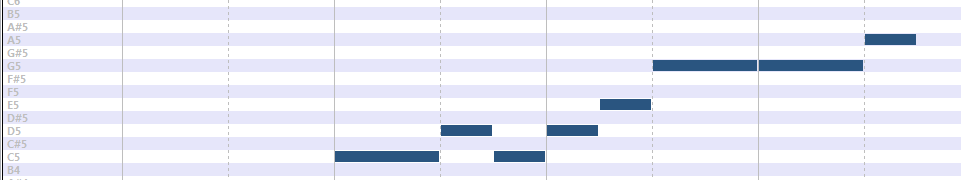
\includegraphics[width=\textwidth]{pianoroll_example}

\paragraph{Modern Western Music Notation (Standard Music Notation, Score)}
\index{Score}
\index{Standard Music Notation}
\index{Modern Western Music Notation}

Modern western music notation is based on five lines representing pitches. Different symbols are used for representing notes based on the duration of the note. All note symbols contain an ellipsoid that is either placed between two of the lines or touching one of the lines. Standard music notation may contain additional information such as \textit{accidentals}, different \textit{clefs}, agoic and several more that are not relevant in the context of this project. The following example shows the same melody notated in standard music notation.

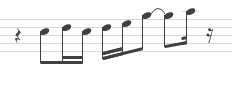
\includegraphics[width= 0.4 \textwidth]{score_example}

Standard music notation will be referred to as \textit{Score} throughout the text.

\paragraph{Tablature}
Tablature is a simpler form of musical notation for string instruments. It has been developed prior to modern western musical notaion but has only gained a high degree of popularity throughout the last decades.

Tablature is based on a variable number of lines representing the string of the instrument. Numbers on the lines represent fret numbers.
Note that:
\begin{itemize}
	\item{Tablature typically does not feature any rhythmic information.}
	\item{On string instruments most notes can be played in more than one position of the fretboard. Tablature provides information on \textit{where} to play a certain note rathern than what note to play.}
\end{itemize}

The following example shows the same melody as above notated in tabulature for a six-string guitar.

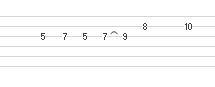
\includegraphics[width= 0.4 \textwidth]{tab_example}

\section{Playing Techniques}
This section treats common playing techniques that are displayed, recognized and evaluated by the application. Emphasis is given to techniques relevant to string instruments.

\subsection{Transitions between Notes}
\paragraph{Bending}
\index{Bending}
Pulling a string upwards or downwards while playing a note causes the pitch to increase. In most situations strings are bent with the intention to raise the pitch of the note by a tone or a semitone.

\paragraph{Slide}
\index{Slide}
Moving the fretting finger up or down the neck of a string instrument while a note rings results in a smooth transition between two notes. This is referred to as \textit{sliding}.

\paragraph{Hammer On / Pull Off}
\index{Hammer On}
\index{Pull Off}
Similarly to slides, \textit{Hammer On}s and \textit{Pull Off}s are smooth transitions between notes. A Hammer On is executed by hammering on the fret, causing the note to sound without plucking the string with the right hand. Similarly a Pull Off is executed by pulling the string away from the fretboard while another finger is used for fretting the note.
\chapter{Technologies}
\label{chap:Technologies}
In this chapter we describe the technologies we have used for this project in detail. 
An overview of these technologies is given here:

\begin{itemize}
	\item Qt, a platform-independent framework for display and audio output.
	\item \gls{MIDI} to read input from instruments like keyboards.
	\item The libraries RtMIDI and libUSB to read MIDI from USB devices.
	\item We read scores from GP5 files.
	\item For audio synthesis we used SoundTouch.
	\item KissFFT provides simple frequency analysis functions for the audio analysis.
\end{itemize}

Qt is a cross-platform application framework written in \cpp from \emph{Digia}. It provides functions for GUI design via QML (see \ref{sec:QML}) and a signal-/slot-concept detailed next.

\section[Qt Signal-/Slot-concept \textsuperscript{Kugler}]{Qt Signal-/Slot-concept}
\label{sec:Signal-/Slot}

The Qt framework provides a signal/slot-concept to allow communication between classes in a thread-safe manner. Classes that inherit from {\tt QObject} can define signals and slots.

\subsection{Signals}

Signals are events other objects can listen to. 
They are defined in the class header after the {\tt signal} keyword.

\begin{lstlisting}
	class SignalExample : public QObject
	{
		Q_OBJECT
		
		public:
			// some variables
			
		signal:
			void mySignal(int someNumber);
	}
\end{lstlisting}

This class has a signal {\tt mySignal} with an integer argument. It can be emitted in a function with the emit keyword like this:

\begin{lstlisting}
	emit mySignal(5);
\end{lstlisting}

\subsection{Slots}

Similar to signals we can define slots using the {\tt slot} keyword. Slots can be specified public or private by using the corresponding keyword.

\begin{lstlisting}
	class SlotExample : public QObject
	{
		Q_OBJECT
		
		public:
			// some variables
			
		public slot:
			void mySlot(int someNumber);
	}
\end{lstlisting}

Slots have a function body that can be triggered by signals. They are defined like normal function implementations.

\begin{lstlisting}
	void SlotExample::mySlot(int someNumber) 
	{
		// do something with someNumber
		cout << someNumber << endl;
	}
\end{lstlisting}

\subsection{Connections}

To use the signals and slots we just created we can connect them by using the {\tt connect} function. 

\begin{lstlisting}
	SignalExample *signalObject = new SignalExample();
	SlotExample *slotObject = new SlotExample();

	connect(
		signalObject, &SignalExample::mySignal, 
		slotObject, &SlotExample::mySlot);
\end{lstlisting}

Now {\tt mySlot} will be called every time {\tt mySignal} is emitted. A signal can be connected to multiple slots and a slot can be connected to multiple signals. 

This mechanism provides a way for objects to communicate with each other and to write highly reusable code. 

\section[QML \textsuperscript{Novotny}]{QML}
\label{sec:QML}
QML is a markup language for defining user interfaces. It is part of the QtQuick framework. QML is loosely based on JSON. The basic structure of the language is declarative. JavaScript can be used inside a QML file which allows including imperative code in the user interface definition. This approach allows implementing both appearance and logic of the user interface in QML rather than \cpp. This section gives an overview of the basic functionalities of QML. Emphasis is given to features relevant to the application.
\subsection{Basics}
\paragraph{QML Components}
QML Components are specified by their type followed by a pair of braces. A QML component may contain child objects. These child components are defined within the braces. Furthermore every component has a set of properties that can be read and modified by other components. Values can be assigned to the properties between the two braces.
\paragraph{Properties}
The values of properties can be either primitive types or QML components. Basically there are two ways to set the value of property.
\begin{itemize}
\item{
	\textbf{Property Bindings}
	Whenever a property is assigned a JavaScript expression inside the definition of the component a property binding is created. This means that the value of the property will be updated automatically if a property included in the expression is updated. This allows specifying property values in a declarative way.
	\begin{lstlisting}
	  Text {
	      text: model.modelData.getTitle()
	      color: standardFontColor
	      font.bold: highlighted
	      font.pixelSize: standardFontPixelSize * 3
	      elide: Text.ElideRight
	      width: scoreDataItem.width  - 2 * marginInItem
	      font.family: headerFont
	  }
	\end{lstlisting}
	A number of property bindings are created in the code examples above. For example:
	\begin{itemize}
		\item {The {\tt text}-property is bound to the result of the function {\tt getTitle} of the property {\tt model.modelData}. The function {\tt getTitle()} will be evaluated when the property {\tt modelData} is updated.}
		\item{The {\tt color}-property of the {Text-} component is bound to the property {\tt standardFontColor} of a parent component.}
	\end{itemize}
}
\item {
	\textbf{Property Assignment}
	The value of a property can be set manually using JavaScript code. Manually setting the value of a property removes any existing bindings of the property.
	\begin{lstlisting}
		Rectangle {
		  Component.onCompleted: {
		      width = parent.width
		  }
		}
	\end{lstlisting}
	In the code example above the {\tt width} -property of the rectangle is set to the current value of the {\tt width} -property of its parent. The property will not be updated automatically if the parent component is updated.
}
\end{itemize}
\subsection{User Input}
\subsubsection{Handling Mouse Events}
QML provides an invisible component called {\tt MouseArea} which inherits {\tt Item}. {\tt MouseAreas} are positioned within other components in order to implement mouse handling. {\tt MouseArea} provides a number of signals such as:
\begin {itemize}
	\item{{\tt onEntered}}
	\item{{\tt onExited}}
	\item{{\tt onClicked}}
	\item{{\tt onDoubleClicked}}
\end{itemize}
\begin{lstlisting}
	Rectangle {
	    width: 100
	    height: 100

	    MouseArea {
	        anchors.fill: parent
	        onClicked: {
	            // Do Something
	        }
	    }
	}
\end{lstlisting}
The position of the mouse cursor can be retrieved via the properties {\tt mouseX} and {\tt mouseY}.
{\tt MouseArea} allows modifying the appearance of the mouse cursor inside the component.
\subsubsection{Handling Key Events}
All QML components provide a property {\tt Keys} to support key handling. This property provides the signals {\tt onPressed} and {\tt onReleased}.
	\begin{lstlisting}
		Rectangle {
	     	Keys.onPressed: {
		         if (event.key === Qt.Key_Return) {
		             event.accepted = true;
		             // Do something
		         }
	     	}
		}
	\end{lstlisting}
Note that by default the event will be forwarded to the parent element. This can be avoided by \textit{consuming} the event which is achieved by setting its {\tt accepted} -property to {\tt true}.
\subsection {Dynamically loading Components}
\paragraph{Loader}
The {\tt Loader} element allows dynamic loading of a subtree of QML objects. {\tt Loader} inherits {\tt Item} and can therefore be used in the same way. \\
This is used to load other QML objects on demand rather than when the application is started.  This leads to serious performance improvements when multiple complex objects need to be loaded at different points in time. 
\paragraph{}
The {\tt Loader} component can load a QML file. This has been used for implementing the application´s menu structure. \\
Alternatively it can load an existing QML object. This has been used in the implementation of  {\tt SelectableListView}, a powerful, flexible {\tt ListView} implementation and will be explained at a later point.
If the source of the Loader is changed the previously loaded Item is destroyed and resources are freed.
\subsection {ListView}
{\tt ListView}s in QML display data provided by data models.

% http://qt-project.org/doc/qt-5/qtquick-modelviewsdata-modelview.html
% 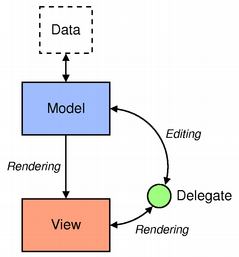
\includegraphics[width=0.5\textwidth]{model_view}

They are highly flexible in terms of what data is displayed and how the data is displayed.
\subsubsection{Data Models}
What data is displayed is determined by data models.
These models can be defined in three ways.
\begin {itemize}
	\item {
		\textbf{QML, by inheriting ListModel} \\
		A ListModel in QML is a source of data. It consists of {\tt ListElements} which can be added dynamically to the list model. The attributes of the ListElements are defined dynamically when creating the records. \\
		These attributes are referred to as data roles. The following code example shows the definition of the list model behind the Display Option Control in the Game Start menu. The contents of the ListModel are specified explicitly inside its definition. The ListElements consist of a single role called \textit{name}.
		\begin{lstlisting}
			ListModel {
               id: displayOptionsModel
               ListElement { name: "Piano Roll"  }
               ListElement { name: "Score" }
               ListElement { name: "Tabulature"}
          	}
		\end{lstlisting}
	}
	\item {
		\textbf{\cpp, as a collection of string values} \\
		This has been used for representing lists of scalar data such as the instrumental tracks contained in a score.
	}
	
	\item {
		\textbf{\cpp, as a collection of QObjects}
		This has been used for representing lists of complex data such as scores and sections inside scores.	
	}
\end {itemize}
\subsubsection {Delegates}
Delegates represent the elements of a view visually. Each record in a view´s model is visualised by the template defined in the delegate. The data of the record can be accessed and modified by its delegate. The delegate may bind to the data roles of its associated record. If the name of a data role coincides with the name of a property of the delegate it can be accessed using the qualified model name instead. If the record is scalar it´s data may be accessed by using the property modelData. 
This feature helps making delegates reusable. 

\subsection{Communication between \cpp and QML}
Due to the tight integration of the Qt Meta Object System in QML passing data to QML objects takes little effort in most situations. Properties, methods and signals of a {\tt QObject} can be accessed from QML.

\subsubsection{Context Properties}
Context properties allow passing data obtained by \cpp code to QML components. Context properties affect all QML objects that are displayed by an {\tt ApplicationView} object. 

The following code examples show how a {\tt QObject} is passed to an {\tt ApplicationView} object as a context property and then used by a QML object.
\begin{lstlisting}
	class DataClass : public QObject
	{
	    Q_OBJECT
	
	    Q_PROPERTY(int number READ getNumber WRITE setNumber NOTIFY numberChanged)
	}
\end{lstlisting}
\begin{lstlisting}
	QQuickView view;
	view.show();
	QPointer<DataClass> data = new DataClass();
	view.rootContext()->setContextProperty("data", data);
\end{lstlisting}

\begin{lstlisting}
	Text {
		anchors.fill: parent
	    text: data.number
	}
\end{lstlisting}

\subsubsection{Making Data Accessible}
Objects passed to QML need to be instances of a class inheriting {\tt QObject}.
Basically there are two ways to make the data of an object available to QML objects:

\begin{itemize}
	\item{Properties}
	\item{Functions}
\end{itemize}

\paragraph{Properties}
In order to be accessible for QML objects class attributes can be wrapped in {\tt Propertie}s.
A property is a wrapper for class attributes. It is associated with a getter method,  an optional setter method and an optional signal that is emitted when the value of the property is changed.
Properties are defined using the {\tt Q\_PROPERTY} macro.

The following code example shows an extract of the definition of a class that uses properties to expose data to QML objects.
\begin{lstlisting}
	class Note : public QObject
	{
	    Q_OBJECT
	
	    Q_PROPERTY(int time READ getTime WRITE setTime NOTIFY timeChanged)
	    Q_PROPERTY(int duration READ getDuration WRITE setDuration NOTIFY durationChanged)
	    Q_PROPERTY(int pitch READ getPitch WRITE setPitch NOTIFY pitchChanged)
	
	private:
	    int time; // number of miliseconds since the song started, 0 if unknown
	    int duration; // 0 if the note is still playing
	    int pitch; // as specified by the MIDI standard, -1 if unknown, 0 is a valid pitch in MIDI

	public:
	    int getTime() const;
	    int getDuration() const;
	    int getPitch() const;
	
	public slots:
	    void setTime(int value);
	    void setDuration(int value);
	    void setPitch(int value);
	
	signals:
	    void timeChanged(int value);
	    void durationChanged(int value);
	    void pitchChanged(int value);
	};
\end{lstlisting}

\paragraph{Functions}
When used in front of the definition of a function the macro {\tt Q\_INVOKABLE} registers a function with the meta-object system. This allows invoking the function from a QML context. 
\subsubsection{Data Type Conversion}
When data is passed from a \cpp context to a QML context it needs to be converted to JavaScript data types. The QML engine will automatically convert most \cpp data types. For example a {\tt QString} object will be converted to a JavaScript string object when passed to a QML object and vice-versa.

\paragraph{Conversion of Custom Types}
Custom Types can be converted to JavaScript types if:
\begin {itemize}
	\item {the class extends {\tt QObject} and}
	\item {the custom type is registered with the QML type system.}
\end {itemize}


\section[Display methods in Qt \textsuperscript{Novotny}]{Display methods in Qt}
Qt provides multiple different ways to display graphics on the screen. Each has different advantages.

\subsection{Inheriting QQuickItem}
Custom components can be created using \cpp by extending the class {\tt QQuickItem}.
{\tt QQuickItem}s are painted using the scene graph approach (explained below).
This approach to drawing custom components has only been introduced with Qt 5. The official documentation lacks examples and detailed explanations. Refer to the presentation \textit{Integrating QML with C++} \cite{qtquickpainting1} by \textit{Digia Plc.} for a brief introduction to the topic.
\subsubsection{Qt Quick Scene Graph}
Traditionally, drawing of custom components in Qt has been based on imperative painting. Imperative painting causes a large amount of draw calls which has a negative affect on the drawing performance.

The scene graph concept has been introduced with Qt 5. The scene graph consists of nodes that are defined before the drawing process is started. This allows a number of optimizations and reduces the number of draw calls significantly.

\subsubsection{Nodes}
Nodes are parts of the scene graph. They represent objects that will be drawn. Node can be containers for other nodes. 

All node classes extend {\tt QSGNode}.
Subclasses used in the project will be discussed in detail.

\paragraph{Memory Managment}
The flag {\tt QSGNode::OwnedByParent} passes ownership of a node to its parent node. The nodes will be deleted as soon as the scene graph is destroyed. Setting this flag is highly recommended in most situations.

Similarly, material and geometry (refer to the explanation below) should be owned by the corresponding node in most situations. This is achieved by using the flags {\tt QSGNode::ownsMaterial} and {\tt QSGNode::ownsNode}.

\paragraph{QSGGeometryNode}
The {\tt QSGGeometryNode} class is the most important node class for drawing custom components. Many other classes such as {\tt QSGSimpleRectNode} extend {\tt QSGGeometryNode}.

A {\tt QSGGeometryNode} primarily consists of 
\begin {itemize}
	\item {Geometry}
	\item {Material}
\end {itemize}

The geometry of a node defines its position, shape and size. The simplest way of specifying the geometry of a node is defining its vertices.

The material defines how a node is filled.

The following code example shows how a line-shaped {\tt QSGGeometryNode} is created.
This example demonstrates how ownership flags are used to ease memory managment.

\begin{lstlisting}
QSGNode* QQI_Based_Visuals::getLineNode(qreal x0, qreal y0, qreal x1, qreal y1, QColor color) {
    QSGGeometryNode* lineNode = new QSGGeometryNode();
    QSGGeometry* lineGeometry = new QSGGeometry(QSGGeometry::defaultAttributes_Point2D(), 2);
    lineGeometry->setLineWidth(2);
    lineGeometry->setDrawingMode(GL_LINE_STRIP);
    lineNode->setGeometry(lineGeometry);
    QSGFlatColorMaterial* material = new QSGFlatColorMaterial();
    material->setColor(color);
    lineNode->setMaterial(material);

    QSGGeometry::Point2D *vertices = lineGeometry->vertexDataAsPoint2D();
    vertices[0].x = x0;
    vertices[0].y = y0;
    vertices[1].x = x1;
    vertices[1].y = y1;

    lineNode->setFlag(QSGNode::OwnedByParent);
    lineNode->setFlag(QSGNode::OwnsGeometry);
    lineNode->setFlag(QSGNode::OwnsMaterial);
    return lineNode;
}

\end{lstlisting}

\paragraph{QSGSimpleRectNode}
{\tt QSGSimpleRectNode} inherits {\tt QSGGeometryNode}. It allows creating rectangle-shaped nodes while simplifying the definition of the geometry. 
{\tt QSGSimpleRectNode} offers a constructor accepting a {\tt QRectF} object.

\begin{lstlisting}
	QRectF noteRectangle = QRectF(left, top, width, height);
	QSGSimpleRectNode* newRectNode = new QSGSimpleRectNode(noteRectangle, Qt::black);
\end{lstlisting}

\paragraph{QSGSimpleTextureNode}
{\tt QSGSimpleTextureNode} simplifies drawing textured objects. A {\tt QSGSimpleTextureNode} primarily consists of 
\begin{itemize}
	\item{texture}
	\item{bounding rectangle}
\end{itemize}

\begin{lstlisting}
	QSGSimpleTextureNode *digitNode = new QSGSimpleTextureNode();
	digitNode->setTexture(digitTextures[digits[i]]);
	digitNode->setRect(left + i * size, top, size, size);
	node->appendChildNode(digitNode);
\end{lstlisting}

\subsubsection{Painting Process}
{\tt QQuickItem} provides the function {\tt update} which causes repainting of the item. 
When the {\tt update} function is called the virtual function {\tt updatePaintNode} is called prior to the rendering process. 

The function {\tt updatePaintNode} receives a {\tt QSGNode} containing the contents of the scene graph at the time the function is called. Th
is allows a more efficient painting process in case only minor changes are made to the graph.

\subsection{Qt Quick Canvas Painting}
The QML {\tt Canvas} component allows painting custom components using Java Script code. 
{\tt Canvas} provides an empty area to draw on.

The {\tt Canvas} component implements the \textit{W3C HTML 5 Canvas} specification. This allows porting HTML 5 canvas components to QML with little effort. 

The article \textit{Qt Quick Painting using Canvas Item} \cite{qtquickpainting2} provided by \textit{Nokia} contains examples and best practices for using the canvas-based drawing approach.

\subsubsection{HTML5 Canvas Specification}
The canvas specification defines a set of drawing commands.
The most important commands include:
\begin{itemize}
	\item{{\tt beginPath} creates a new {\tt path}}
	\item{{\tt moveTo}}
	\item{{\tt line} adds a line-shaped path defined by the supplied coordinates}
	\item{{\tt rect} adds a rectangle-shaped path defined by the supplied coordinates}
	\item{{\tt text} adds a path consisting of text in a specific font}
	\item{{\tt stroke} draws the path}
\end{itemize}

\subsubsection{Canvas-Based Drawing in QML}
The {\tt Canvas} element provides the signal {\tt onPaint} which is emitted whenever repainting of the component is requested. 

The following example is an extract of the JavaScript-based implementation of the {\tt TabatureView} component. It demonstrates the canvas-based drawing process. Note that the component has been reimplemented using the {\tt QQuickItem}-based drawing approach due to performance issues.

\begin{lstlisting}
Canvas {
	id: canv
    anchors.fill: parent
    onPaint: {
        doTheDrawing(canv.context);
    }
    
    function drawLine(ctx, xFrom, yFrom, xTo, yTo, color, strength) {

        ctx.moveTo(xFrom, yFrom);
        ctx.lineTo(xTo, yTo);
        ctx.strokeStyle = color;
        ctx.lineWidth = strength;
        ctx.stroke();
    }
    
    function doTheDrawing(ctx) {
    
        for(var i = 1; i <= tabulatureView.numOfStrings(); i++) {
            drawLine(ctx, 0,  getStringLevel(i), canv.width, getStringLevel(i), "#000000", 1);
        }
 	}
}
\end{lstlisting}

As opposed to the {\tt QQuickItem}-based drawing approach the {\tt Canvas} painting approach does not make use of a scene graph which negatively affects performance when painting complex components. Performance problems occur especially in real-time applications.

\section[The MIDI protocol \textsuperscript{Kugler}]{The MIDI protocol}
\gls{MIDI} is a protocol to describe time-coded events. It is commonly used to transfer music notes from electronic instruments to computers and synthesizers. An important part of the project is to let people play with real instruments. With \gls{MIDI} we can read what keys the user plays from MIDI instruments like keyboards.

\subsection{Overview}
\gls{MIDI} serially transmits messages with a fixed size of 8 bit at a fixed rate. The first bit of a message determines whether the next 7 bits are a status code or data. The first 3 bit of the status code define the type of the message, the next 4 bit the channel. Therefore \gls{MIDI} supports up to 16 different channels. Devices can be set up to only listen to a specific channel. A status message is followed by up to two data messages, defining parameters of the status.

The most important messages are 
\begin{description}
	\item[Note-On] \hfill \\ Activates a note and contains information about pitch and volume.
	\item[Note-Off] \hfill \\ Deactivates the note.
	\item[Control Change] \hfill \\ Changes one of the 128 user-defined parameters. Most synthesizers allow configuration of how these values are interpreted.
	\item[Program Change] \hfill \\ Sets the program number for this channel. These define which instrument/synthesizer should play the notes.
\end{description}

MIDI can be transmitted over MIDI cables or encapsulated in other data streams over USB, FireWire, Ethernet, etc.
Beat the Score only supports MIDI over USB as standard MIDI connectors are rare nowadays. For the communication with MIDI devices libUSB and RtMidi have been used (see section \ref{sec:libusb and RtMidi}).

\subsection{General MIDI specification}
Since MIDI itself does not give any meaning to the program and control numbers the general midi standard has been created. The general MIDI specification defines for each of the 128 program numbers an instrument. Those range from different pianos, guitars and strings to synthetic sounds. For percussion the channel 10 is reserved and a percussion instrument is assigned to each pitch number. 


\section[GP5 Format \textsuperscript{Kugler}]{GP5 Format}
\label{sec:GP5}
To support many play techniques we decided to use the Guitar Pro 5 format, a proprietary file format developed by \emph{Arobas Music}. It is specialized for guitars but supports other instruments as well. 

This section uses the vocabulary described in chapter \ref{chap:Basic Musical Terms}.

Other than MIDI, it stores multiple additional informations, including but not limited to
\begin{itemize}
	\item number of strings on the guitar and tuning,
	\item how a string is picked,
	\item whether the note has been played as a harmonic note and if, what kind of harmonic note,
	\item what fingers are used to grip the an accord.
\end{itemize}

This information is used to display and detect notes more accurately for guitars.

Another big advantage is that songs in the GP5 format can be found in vast amounts on the internet.

The file consists of five parts:
\begin{enumerate}
	\item Meta information
	\item Song data
	\item Bars
	\item Track
	\item Beats
\end{enumerate}

\subsection{Meta information}

This contains information about the song and the score:
\begin{itemize}
	\item song title and subtitle
	\item name of the interpret
	\item name of the album
	\item name of the composer
	\item name of the transcriber
	\item page setup
\end{itemize}

\subsection{General song information}

Information about the actual song: 
\begin{itemize}
	\item tempo of the song
	\item signature
	\item the General MIDI instrument number for each track
\end{itemize}
		
\subsection{Bars}

This part contains an entry for every bar of the song and stores information about
\begin{itemize}
	\item signature changes
	\item information about repetition
	\item names and positions of the sections
\end{itemize}

\subsection{Track}

For every instrument in the song, additional information is stored. If the instrument is a guitar this sections contains how many strings are used and how they are tuned.

\subsection{Beat}

The actual notes for every bar and track. Informations stored here are:
\begin{itemize}
	\item length of the beat
	\item pitch (or pitches if an accord is played) of the beat
	\item information about bending
	\item linking to the next note
\end{itemize}

\section[SoundTouch \textsuperscript{Neumayer}]{SoundTouch}
\label{sec:SoundTouch}
To pitch missing audio samples from existing Wave files ({\tt .wav}) Beat The Score uses the SoundTouch library. In this section we describe how to use the SoundTouch library for pitching audio samples.
\subsection{Usage}
\begin{enumerate}
\item Create a {\tt SoundTouch} object and set predefined settings. In this example we choose to use the much faster quick seeking algorithm in SoundTouch's internal tempo changer routine and disable it's anti-aliasing filter. Changing the default settings results in dramatically faster pitching on ARM processors as CPU utilization is lowered.
\item Read a sound file (RIFF WAVE format) into memory and store a pointer to its data as {\tt tmpBuf} as well as the size of the {\tt char[]} behind that pointer. Note, the {\tt f.seek(44);} instructs the {\tt QFile} object to skip the WAVE file's RIFF header, it's format section as well as the data's header signature and the data length field, which results in a size of 44 bytes, according to the Wikipedia article about the RIFF WAVE format (http://de.wikipedia.org/wiki/RIFF\_WAVE).
\item Set by how many semi-tones the audio sample should be pitched. A positive value indicates pitching the sample up where as a negative value indicates pitching the sample down.
\item Put the to-be-pitched audio sample into SoundTouch's internal buffer and flush remaining samples from the buffer if available.
\item Create a new block of memory for storing the result of the pitching process. In the example the pointer {\tt newSample} points to this memory block. Since we have configured the SoundTouch library (at compile time) to use integer samples {\tt SAMPLETYPE} is a typedef to a \cpp {\tt short} type which has a size of 16 bits. In contrast, a \cpp {\tt char} has a size of 8 bits. This is the reason for both casting between {\tt SAMPLETYPE}s and {\tt char}s as well as multiplying SoundTouch's internal sample size by 2 for the new audio sample memory. The size of these types depends on the processor architecture but it applies to the main target architectures, x86 and ARM. Afterwards we pull the pitched data from SoundTouch's internal memory buffer into our newly created {\tt newSample}.
\end{enumerate}

\begin{lstlisting}
// Step 1
SoundTouch st;
st.setChannels(1);
st.setSampleRate(44100);
st.setSetting(SETTING_USE_QUICKSEEK, 1);
st.setSetting(SETTING_USE_AA_FILTER, 0);

// Step 2
QFile f(QString("test.wav"));
f.open(QIODevice::ReadOnly);
f.seek(44);
QByteArray barr = f.readAll();
f.close();
char * tmpBuf = barr.data();
int tmpBufSize = barr.size();

// Step 3
st.setPitchSemiTones(1);

// Step 4
st.putSamples((SAMPLETYPE*)tmpBuf, tmpBufSize);
st.flush();

// Step 5
int numSamples = st.numSamples();
int newSampleSize = numSamples * 2; // numSamples = number of 2 byte samples
char *newSample = new char[newSampleSize];
st.receiveSamples((SAMPLETYPE*)newSample, numSamples);
st.flush();
\end{lstlisting}


\section[KissFFT \textsuperscript{Kugler}]{KissFFT}
\label{sec:KissFFT}
The KissFFT library provides an implementation of the \gls{FFT} for frequency analysis. Here we describe how to use the library. See chapter \ref{chap:Audio analysis} for how we use the library to detect notes in audio signals.

\subsection{Usage}
To transform a signal from time domain into frequency domain we follow these steps:
\begin{enumerate}
	\item Create a {\tt kiss\_fft\_cfg} with the size of the signal. This will calculate all parameters for the given size. Most of the time you will always analyse the same number of samples so this object can be reused. Note that the size of the signal has to be a power of two.
	\item Write the signal into a {\tt kiss\_fft\_cpx} array. Hence we are dealing with real numbers and not complex ones, we just set the complex part of the entries to 0.
	\item Call the {\tt kiss\_fft} function with the configuration from step 1, the {\tt kiss\_fft\_cpx} array and a second {\tt kiss\_fft\_cpx} array for the result. Note that in-place calculation is not supported. If the same array is provided as input and output the function will create another buffer and write it back when the calculation finished.
\end{enumerate}

\begin{lstlisting}
	int fftSize = 1024;
	float *signal = new float[fftSize];

	// Step 1
	kiss_fft_cfg fftConfig = kiss_fft_alloc(fftSize, 0, NULL, NULL);
	
	// Step 2
	kiss_fft_cpx *complexSignal = new kiss_fft_cpx[fftSize];
	for (int i=0; i<fftSize; i++)
	{
		complexSignal[i] = (kiss_fft_cpx){signal[i], 0};
	}
	
	// Step 3
	kiss_fft_cpx *frequencySpectrum = new kiss_fft_cpx[fftSize];
	kiss_fft(fftConfig, complexSignal, frequencySpectrum);
	
	// frequencySpectrum contains now the result
	
	// cleanup
	delete complexSignal;
	delete signal;
	delete frequencySpectrum;
\end{lstlisting}

\subsection{Interpretation of the result}
The result contains the amplitude and phase for each sine component of the signal. We can calculate the index at which a given frequency can be found with
$$ i = f \frac{N}{samplerate} $$
where $i$ is the index in the result array, $f$ the frequency we are looking for, $samplerate$ the samplerate of the signal and $N$ the number of samples in the signal.

Because of the Nyquist-Shannon sampling theorem the frequencies above $\frac{N}{2}$ contain the same values as the lower half mirrored. They are not interesting for us.

The length of the complex entries describe the amplitude of the sine waves and the orientation describe the phase. Thus we can calculate the values using the trigonometry functions provide by {\tt math.h}.
\begin{lstlisting}
	float amplitude = hypotf(frequencySpectrum[index].r, frequencySpectrum[index].i);
	float phase = atan2f(frequencySpectrum[index].r, frequencySpectrum[index].i);
\end{lstlisting}


\section[libusb and RtMidi \textsuperscript{Neumayer}]{libusb and RtMidi}
\label{sec:libusb and RtMidi}

\subsection{RtMidi}
On desktop systems the way to handle MIDI signals happens through the RtMidi library. 
RtMidi uses the operating systems audio subsystem to get a list of connected MIDI devices and receive signals from them. On Windows RtMidi uses the Microsoft Multimedia MIDI API while on Linux it uses the Advanced Linux Sound Architecture API. The use of APIs for the respective platform is set at compile time of the RtMidi library.

\subsection{libusb}
As one of our goals was to make Beat The Score work on multiple platforms using the same code base we had to make sure that giving input to the application worked on all supported platforms in a similar way. To accomplish that on Android, we had to switch the library for receiving MIDI data as most Android devices do not have ALSA MIDI support enabled at the kernel level.
\\
The Android version of Beat The Score uses libusb instead of RtMidi to read data from the connected USB MIDI input device. We use a specially modified version of libusb which is forked from github.com/SpecLad/libusb-android. The forked version is available at github.com/beatthescore/libusb. The Android version of libusb allows the use of file descriptors to open the USB device through the Linux kernel. Since Android uses a fairly standard Linux kernel it works the same as other typical Linux systems where devices are represented as virtual files on the filesystem. To open the file descriptor of the USB device we use Java code in the form of broadcast receivers which asks the Android framework to open the file and return the file descriptor. The Java code is mandatory as there are no documented APIs that allow gaining the required permissions using purely native code.
\\
The way Android allows applications to access USB devices is by reading in the application's manifest file ({\tt AndroidManifest.xml}) and checking if the application requests the permission to access USB devices. On Android the user permits applications the required permissions at install time. The following code snippet specifies the request for the permission.
\begin{lstlisting}
<uses-feature android:name="android.hardware.usb.host"/>
\end{lstlisting}

When the application is started it has to register a so-called broadcast receiver that gets triggered when certain events happen on the system. An {\tt IntentFilter} is required to make the application only react to events that are relevant.
\begin{lstlisting}
IntentFilter filter = new IntentFilter(JNIUtils.ACTION_USB_PERMISSION);
registerReceiver(JNIUtils.UsbReceiver, filter);
\end{lstlisting}

This registers a receiver that only should be triggered when a USB device is connected.
\\
When the broadcast receiver is triggered it checks whether the user actually allowed the application to open the device. The following broadcast receiver resides in the {\tt JNIUtils} Java class.
\begin{lstlisting}
public static final BroadcastReceiver UsbReceiver = new BroadcastReceiver() {

public void onReceive(Context context, Intent intent) {
  if (ACTION_USB_PERMISSION.equals(intent.getAction())) {
    synchronized (context) {
      UsbDevice device = (UsbDevice)intent.getParcelableExtra(UsbManager.EXTRA_DEVICE);
	  if (intent.getBooleanExtra(UsbManager.EXTRA_PERMISSION_GRANTED, false)) {
        if(device != null) {
          UsbDeviceConnection conn = usbManager.openDevice(device);
          int descriptor = conn.getFileDescriptor();
          setConnected(device.getVendorId(), device.getProductId(), endPointAdr, descriptor);
        }
      } else {
        Log.d("BTS", "permission denied for device " + device);
      }
    }
  }
}
};
\end{lstlisting}

The call to {\tt setConnected()} actually is a JNI call to native code.

\begin{lstlisting}
extern "C" {
  JNIEXPORT void JNICALL Java_at_beatthescore_JNIUtils_setConnected(JNIEnv * env, jobject obj,
    jint vendorId, jint productId, jint endpoint, jint descriptor);
  JNIEXPORT void JNICALL Java_at_beatthescore_JNIUtils_setConnected(JNIEnv * env, jobject obj,
    jint vendorId, jint productId, jint endpoint, jint descriptor)
  {
    usbVendorid = (int)vendorId;
    usbProductid = (int)productId;
    usbDescriptor = (int)descriptor;
    usbEndPoint = (int)endpoint;
  }
}

\end{lstlisting}
This exposes the native \cpp function to the Java-part of the Android application through JNI (Java Native Interface). 
The following values have to be provided to {\tt setConnected()} for the native code to allow using the USB device.

\begin{description}
\item[Vendor and product identifier:] \hfill \\ These values are used to get the right {\tt libusb\_device} object.
\item[The USB device's end point:] \hfill \\ As USB devices can have multiple end points for data transmission the application needs to open the end point that provides the host with MIDI data.
\item[The file descriptor:] \hfill \\ The file descriptor for the USB device (provided by the operating system kernel and passed on to the application by the Android framework)
\end{description}

In order to catch this broadcast event, the application has to register broadcast receivers for dealing with attaching and detaching USB devices to the Android host.

\begin{lstlisting}
public static final BroadcastReceiver ConnectReceiver = new BroadcastReceiver() {

  public void onReceive(Context context, Intent intent) {
    if(intent.getAction().equals(UsbManager.ACTION_USB_DEVICE_ATTACHED))
    {
      UsbDevice device  = (UsbDevice)intent.getParcelableExtra(UsbManager.EXTRA_DEVICE);
      if(device != null) {
        for(int i = 0; i < device.getInterfaceCount(); i++) {
          UsbInterface tmpInterface = device.getInterface(i);
          for(int j = 0; j < tmpInterface.getEndpointCount(); j++) {
            UsbEndpoint endPoint = tmpInterface.getEndpoint(j);

            if(endPoint.getDirection() == 128) { //Direction from device to host
              endPointAdr = endPoint.getAddress();
              PendingIntent mPermissionIntent;
              mPermissionIntent = PendingIntent.getBroadcast(context, 0, new Intent(ACTION_USB_PERMISSION), 0);
              usbManager.requestPermission(device, mPermissionIntent);
            }
          }
        }
      }
    } else if(intent.getAction().equals(UsbManager.ACTION_USB_DEVICE_DETACHED)) {
      setConnected(-1, -1, -1, -1);
    }
  }
};
\end{lstlisting}

As with the {\tt JNIUtils.UsbReceiver} the {\tt JNIUtils.ConnectReceiver} has to be registered to react to broadcast events.

\begin{lstlisting}
connectFilter.addAction(UsbManager.ACTION_USB_DEVICE_ATTACHED);
connectFilter.addAction(UsbManager.ACTION_USB_DEVICE_DETACHED);
registerReceiver(JNIUtils.ConnectReceiver, connectFilter);
\end{lstlisting}

Opening the USB device is done by getting the right {\tt libusb\_device} object in a simple loop followed by opening the device using the provided file descriptor:
\begin{lstlisting}
libusb_device_handle *dev_handle;
libusb_context *ctx = NULL;
libusb_device **devs;
ssize_t cnt;

libusb_init(&ctx);
cnt = libusb_get_device_list(ctx, &devs);
libusb_device *selectedDevice = NULL;
for(i = 0; i < cnt; i++) {
  libusb_device_descriptor desc;
  int r = libusb_get_device_descriptor(devs[i], &desc);
  if (desc.idVendor == this->androidGlue->getVendorID() &&
      desc.idProduct == this->androidGlue->getProductID()) {
    selectedDevice = devs[i];
  }
}
libusb_open2(selectedDevice, &dev_handle, this->androidGlue->getDescriptor());
\end{lstlisting}

Reading data from the devices end point is done by calling {\tt libusb\_bulk\_transfer()}.
\begin{lstlisting}
int ret = libusb_bulk_transfer(dev_handle, this->androidGlue->getEndpoint(), data, 4, &nBytes, 3000);
\end{lstlisting}
The return value of the call allows the application to check whether the data transfer worked as intended. 
{\tt Note} objects will not be generated from the data when the transfer function returns one of the two following errors.
\begin{itemize}
\item LIBUSB\_ERROR\_TIMEOUT
\item LIBUSB\_ERROR\_OVERFLOW
\end{itemize}

\section[OpenSSL \textsuperscript{Neumayer}]{OpenSSL}
\label{sec:OpenSSL}
The license files that allow the use of Beat The Score are generated on the backend of the server side using the OpenSSL cryptographic library. It is also used in the application to validate the license.

The steps to generate a valid and asymmetrically encrypt license using OpenSSL:
\begin{enumerate}
\item Open the private RSA key using {\tt fopen()} and load its contents into memory using {\tt PEM\_read\_RSAPrivateKey()}.

\item Cast the decrypted message from {\tt char*} to {\tt const unsigned char*} as this is what OpenSSL expects as the message's type when encrypting.

\item Encrypt the message using {\tt RSA\_private\_encrypt()}. The method expects the length of the cleartext message, the cleartext message itself, where to store the encrypted message, the private RSA key and the padding of the cleartext message. If the encryption process was unsuccessful, the {\tt bufferSize} will get -1 as its value, otherwise it will get the encrypted messages size.

\item Create a {\tt vector} of {\tt uint8\_t} values out of the encrypted message. This is done because one of the design goals of the backend was to not use pointers between method calls to reduce the risk of memory leaks.

\item Clean up memory and close the open file descriptor to the private key.
\end{enumerate}

\begin{lstlisting}
vector<uint8_t> generateEncryptedMessage(string message, string privateKey) {
    // Step 1
    const char *privkeyPath = (const char*) privateKey.c_str();
    unsigned char *encryptedMessage = new unsigned char[1024]; //should be enough
    FILE *privateKeyFile = fopen(privkeyPath, "r");
    RSA *rsaPrivate = PEM_read_RSAPrivateKey(privateKeyFile, NULL, NULL, NULL);
    if(rsaPrivate == NULL) {
	    RSA_free(rsaPrivate);
	    delete [] encryptedMessage;
    	    fclose(privateKeyFile);
        return vector<uint8_t>();
    }

    // Step 2
    const unsigned char *decryptedMessage = (const unsigned char*) message.c_str();
    
    // Step 3
    int bufferSize = RSA_private_encrypt(message.length(), decryptedMessage,
                                        encryptedMessage, rsaPrivate, RSA_PKCS1_PADDING);
    if(bufferSize == -1) {
        RSA_free(rsaPrivate);
	    delete [] encryptedMessage;
    	    fclose(privateKeyFile);
        return vector<uint8_t>();
    }

    // Step 4
    vector<uint8_t> retVec;
    for(int i = 0; i < bufferSize; i++) {
        retVec.push_back((uint8_t)encryptedMessage[i]);
    }


    // Step 5
    RSA_free(rsaPrivate);
    delete [] encryptedMessage;
    fclose(privateKeyFile);

    return retVec;
}
\end{lstlisting}

To store the encrypted message in a database or to transmit the message through a RESTful web API to the application it is encoded to Base64. The Qt framework provides a simple member method to do that: {\tt QString::toBase64()}. The sample method to decrypt an encrypted message from memory looks similar. The difference is that, on the application side, the public key should not be stored on the persistent storage device of the user as this would allow modifications easily of the public RSA key. Instead, the public RSA key is compiled into the binary of Beat The Score and read from memory. To do this a {\tt static const unsigned char public\_pem[]} is generated out of the public key file before compilation of Beat The Score. This is then used in the decryption method on the client side. {\tt BIO\_new\_mem\_buf} and {\tt PEM\_read\_bio\_PUBKEY} are used in sequence to make the OpenSSL library use the key that is stored inside {\tt public\_pem}. According to the official OpenSSL documentation (https://www.openssl.org/docs/crypto/bio.html), {\tt BIO} in OpenSSL is "an I/O abstraction" and it can be used to "transparently handle SSL connections, unencrypted network connections and file I/O".

\begin{lstlisting}
QString decryptMessage(unsigned char *message, int size)
{
    int pem_size = sizeof(public_pem)/sizeof(*public_pem);
    BIO *publicKeyBuffer = BIO_new_mem_buf((void*)public_pem, pem_size);
    RSA *rsaPublic;
    EVP_PKEY *pkey = PEM_read_bio_PUBKEY(publicKeyBuffer, NULL, NULL, NULL);
    if (pkey) {
        rsaPublic = EVP_PKEY_get1_RSA(pkey);
        if (rsaPublic) {
            RSA_up_ref(rsaPublic);
        }
        EVP_PKEY_free(pkey);
    }
    if(rsaPublic == NULL) {
        return NULL;
    }
    unsigned char *decryptedMessage = new unsigned char[1024];
    int bufferSize = RSA_public_decrypt(size,
                                        message,
                                        decryptedMessage,
                                        rsaPublic,
                                        RSA_PKCS1_PADDING);
    if(bufferSize == -1) {
        return NULL;
    }

    RSA_free(rsaPublic);
    BIO_free(publicKeyBuffer);
    QString retStr((const char*)decryptedMessage);
    delete [] decryptedMessage;
    if(retStr.isEmpty() || retStr.isNull()) {
        return NULL;
    }
    return retStr;
}

\end{lstlisting}

\chapter[Design \textsuperscript{Kugler}]{Design}
\label{chap:Design}
The purpose of this chapter is to give an overview over the implementation design of Beat the Score. This chapter focuses on the communication between the different parts. 

\section{Data structures}

\subsection{{\tt Score}}

The data structure for songs. It consists of meta information about the song such as the title, the interprets and a list of tracks. This structure is used to store the songs from the GP5 files (see section \ref{sec:GP5}) with which the player input is compared to.

\subsection{{\tt Track}}

A {\tt Track} is a line of notes and information about the instrument that plays it. Additionally to the tracks in the {\tt Score}, we also store the player input in a {\tt Track}.

\subsection{{\tt Note}}

To store informations about individual notes. The most important ones are:
\begin{description}
	\item[time] in milliseconds after the start of the song. 
	\item[duration] in milliseconds.
	\item[pitch] as used in the MIDI specification.
\end{description}

\section{Program modules and communication}

For modularity the program has been split up into multiple parts:
\begin{description}
	\item[Inputs] \hfil \\ Handles inputs of an instrument.
	\item[Visuals] \hfil \\ Displays notes.
	\item[Sound] \hfil \\ Synthesizes an audio output.
	\item[Evaluator] \hfil \\ Compares the player input to the actual score and calculates how many points the player receives.
	\item[Main-Game] \hfil \\ Establishes and removes connections between the other parts when necessary. The GUI mostly communicates with this class.
\end{description}

Most communication between the different parts are done over Qt's Signal-/Slot-concept (see section \ref{sec:Signal-/Slot}).

\subsection{Inputs}
This part consists of the superclass {\tt Input} and an implementation for each input method. Scope of the project was only the support for MIDI keyboards over USB ({\tt MidiInput}) and guitars over phone connectors ({\tt AudioInput}, see chapter \ref{chap:Audio analysis}) but support for additional input methods can be added easily. 

\begin{sloppypar}
To create instances of those classes the class {\tt MidiInputManager} and {\tt AudioInputManager} are implemented. The purpose of those is to look for connected hardware of the respective type. 
\end{sloppypar}

{\tt Input} provides the following signals:
\begin{description}
	\item[{\tt noteOn(Note *note)}] \hfil \\ when a note is activated.
	\item[{\tt noteOff(Note *note)}] \hfil \\ when a note is released.
	\item[{\tt notePitchChanged(Note *note, float pitch)}] \hfil \\ when pitch bending is applied to a playing note.
\end{description}

\subsection{Visuals}
This part handles drawing the notes to the screen. It consists of the superclass {\tt Visuals} and its implementations {\tt PianoRoll}, {\tt ScoreView} and {\tt TablatureView}. The subclasses are detailed further in chapter \ref{chap:In-Game User Interface}. 

Additional display options can be added easily.

{\tt Visuals} provides the following slots:
\begin{description}
	\item[{\tt noteOn(Note *note)}] \hfil \\ when the player begins to play a note to make the note flash up in the view.
	\item[{\tt stateChanged(State state)}] \hfil \\ to react to pausing and resuming of the game in the trainings mode.
\end{description}

Further updates to player inputs are not required as an instance of {\tt Visuals} has a pointer to the {\tt Track} the {\tt Evaluator} writes into.

\subsection{Sound}
Responsible for audio output are the classes {\tt MidiNoteOutput} for the player input and {\tt NoteOutput} for the backing track. Both write into an instance of the class {\tt AudioBuffer} which is responsible for the mixing. By splitting it up like that we can avoid playing the notes from instruments that already have an audio output (in the scope of this project only guitars) by simply not connecting the {\tt Input} with the {\tt MidiNoteOutput}. How the synthesis of the audio output works is detailed in chapter \ref{chap:Audio output}.

The class {\tt MidiNoteOutput} has the following slots:
\begin{description}
	\item[{\tt noteOn(Note *note)}] \hfil \\ for when a note is activated.
	\item[{\tt noteOff(Note *note)}] \hfil \\ for when a note is released.
\end{description}

Those slots are compatible to the signals of the {\tt Input}s. Note that there is no corresponding slot for the {\tt notePitchChanged}-signal since we do not support pitch bending for MIDI instruments.

To play the backing tracks it stores a list of pointers to the corresponding {\tt Track} instances.

\subsection{Evaluator}
The linking piece between the inputs and the game. This part only consists of the class {\tt Evaluator} but could be extended by additional play modes in the future. 

The {\tt Evaluator} listens to notes with the slots 
\begin{description}
	\item[{\tt noteOn(Note *note)}] \hfil \\ for when a note is activated.
	\item[{\tt noteOff(Note *note)}] \hfil \\ for when a note is released.
	\item[{\tt notePitchChanged(Note *note, float pitch)}] \hfil \\ when pitch bending is applied to a playing note.
\end{description}
and reacts to them with the signal
\begin{description}
	\item[{\tt noteAdded(Note *note)}]\hfil \\ for further updates on the note, for example when the note is released, corresponding signals will be emitted by {\tt note} itself.
\end{description}

Transforming the stream of {\tt noteOn}- and {\tt noteOff}-signals into a stream of {\tt noteAdded}-signals with and observable {\tt Note} object has the advantage that we don't need to match the {\tt noteOff}-signals to the corresponding {\tt noteOn}-signals and also don't have to deal with notes being \emph{stuck} when the {\tt noteOff}-signal got lost because the object got disconnected from the input. Once the {\tt noteAdded} has been received by an object it can listen to the duration of the note which will be set as soon as the note is released. Even if the listening object got disconnected from the input, it can react to the end of the note properly.

The evaluator is also responsible for matching the player input with the actual score and award points depending on how close the note is to the actual score. The rules here are that the note must be in-key and the starting and ending points must be within a certain radius. If a new note is played which is closer to the actual note than a previously played note the closer one replaces the old on. 

\subsection{Main-Game}
This part consists of a single object of type {\tt MainGame} which is present throughout the whole runtime. It provides signals and properties accessible by the GUI to communicate the state of the game and the GUI calls its functions to control the game. This part only describes the user interactions from the \cpp side, for the QML side see chapter \ref{chap:UI}.

When the program is started the {\tt mainGame} object initializes the input managers and audio outputs and connects the {\tt MidiInput}s with the {\tt MidiNoteOutput} so the user can hear the notes they play already in the menu and to allow note-based navigation (see section \ref{sec:sound based navigation}).

The {\tt mainGame} object provides multiple functions to change the state of the game:
\begin{description}
	\item[{\tt songSelection()}] \hfil \\ to enter the song selection screen. It loads the default settings from the database so the GUI can preselect them.
	\item[{\tt startSong()}] \hfil \\ prepares a song for playing.
	\item[{\tt startAgain()}] \hfil \\ resets the user input so the song can be played again.
	\item[{\tt startReplay()}] \hfil \\ prepares playback of the previous user input.
\end{description}

Some of these states allow usage of additional functions. These are described in the following sections.

\subsubsection{{\tt songSelection()}}
The default settings are loaded from a local database (see section \ref{sec:Preferences}). If the user just played a song when this function is called all data of that song is released and the {\tt MidiInput}s are connected to the {\tt MidiNoteOutput} again (see section \ref{subsec:startSong}).

After this function has been called, multiple functions to change settings of the game can be used:
\begin{description}
	\item[{\tt selectSong(QString filename)}] \hfil \\ loads a song from the disk and prepares song-specific settings like track- and section-selection.
	\item[{\tt selectInput(int index)}] \hfil \\ selects the specified input device.
	\item[{\tt selectTrack(int index)}] \hfil \\ selects the specified track from the song.
	\item[{\tt setTempo(float factor)}] \hfil \\ changes the song to the specified tempo.
\end{description}

\subsubsection{{\tt startSong()}}
\label{subsec:startSong}
This function can be only called after all settings for a song have been set. It sets up the game in the following steps:
\begin{enumerate}
	\item All input devices that aren't used are disconnected. 
	\item A track for the user input is created.
	\item An evaluator is created and connected with the selected input device.
	\item The {\tt NoteOutput} gets a reference to the selected score.
\end{enumerate}

\subsubsection{{\tt startAgain()}}
After the completion of a song the player can choose to play again. To avoid destroying all objects just to create them again this is done with this extra function.

\subsubsection{{\tt startReplay()}}
Like the {\tt startAgain()} function this can be called after a song has been played. It will reset the visual but keep the player input. The inputs are not connected, so it's not possible to play new notes.
\chapter[Audio analysis \textsuperscript{Kugler}]{Audio analysis}
\label{chap:Audio analysis}

A big part of the project is to give players the ability to play with their own instruments. To archive this we had to face a number of problems. 
\begin{itemize}
	\item Bass guitars can play very low notes which frequencies are closer together and therefore are hard to distinguish.
	\item Guitars have many overtones which could be misinterpreted as notes. 
	\item Microphones and sound \glspl{pick-up} vary a lot in sensitivity. It is impossible to find a threshold that works for everybody. 
	\item Microphones have different sensitivity for different frequencies. The input has to be normalized with an equalizer. 
\end{itemize}

To work well for many people all parameters have to be adjusted at runtime dynamically. Therefore the program generates statistics about the characteristics of the audio signal and calculates the parameters for note detection accordingly. 


The algorithm presented here is similar to the on described in \cite{harmo1} in that way that we use what they call \emph{harmonic atoms}. However, for performance reasons we use the generalised Hough transform instead of a matching pursuit to analyse the frequency spectrum. 


To detect notes we use a method called short-time Fourier transformation. The audio signal is processed in the following steps:
\begin{enumerate}
	\item Split up the signal in multiple overlapping slices.
	\item Apply the Hann window function to each slice.
	\item Generate a frequency spectrum for every slice.
	\item Remove noise and apply an equalizer to account for differences in microphones and \glspl{pick-up}.
	\item Apply a scoring function to remove overtones and increase frequency resolution.
\end{enumerate}

Each step is described in further detail in the following sections.

\section{Choice of audio input parameters}
An audio input basically has two parameters. The sample rate, which is the number of times the signal is measured and the bit rate, the accuracy at which signals are measured.
For example, standard audio CDs use a sample rate of 44.1kHz and a bit rate of 16 bit. 
Since higher sample rate leads to a better detection quality the program tries to use the highest option that is available on the system.

\section{Splitting up the input into slices}
In a first step the continuous audio signal is split up into slices, each containing 4096 samples. The more samples are used the more accurate can the frequency be determined. The range in which frequencies can be found can be calculated as
$$ \frac{samplerate}{N} \leq F \leq \frac{samplerate}{2} $$
where $N$ is the number of samples in the slice and $samplerate$ is the number of samples per second of the audio signal. The upper bound results from the Nyquist–Shannon sampling theorem. Because the \gls{FFT} is a divide and conquer algorithm that repeatedly splits up the samples into halves, the number of samples in the buffer have to be a power of 2.

We chose to use a size of 4096 samples. With the common sample-rate of 44.1 kHz this is high enough to accurately detect the lowest notes of bass guitars. 4096 samples are about 0.1 second at this sample-rate. To get a higher time-resolution, the slices overlap each in other in such a way that a new slice begins every 5 milliseconds. Therefore, the samples are written into a ring-buffer which is copied every time enough new samples have been written (see figure \ref{fig:ring-buffer}).

\begin{figure}
	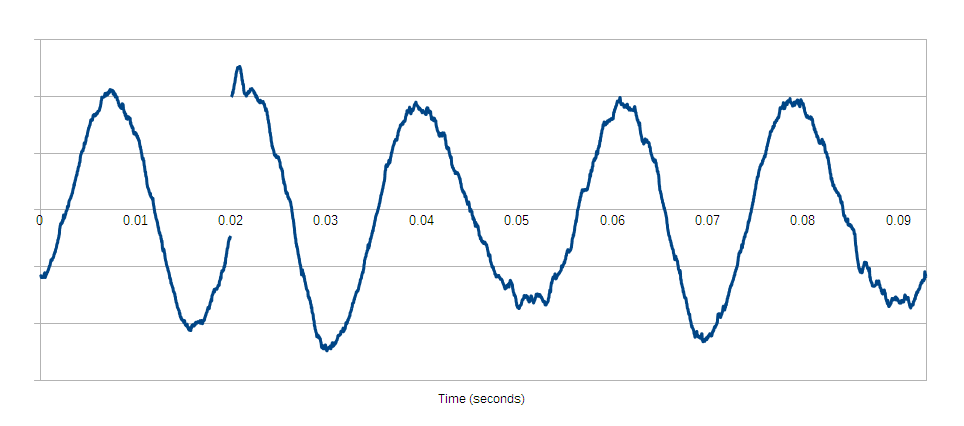
\includegraphics[width=\textwidth]{ring_buffer}
	\caption{An example of the content of the ring-buffer while a bass guitar is playing. Note the point of discontinuity where the new samples are written over the old ones. (Information about the scale of the Y axis is not available as we do not know the sensitivity of the microphone)}
	\label{fig:ring-buffer}
\end{figure}

\section{Hann window function}
The \gls{FFT} interprets the buffer as a repeating signal. To avoid noise that is generated by the point of discontinuity we apply a window function that is zero-valued at that point. 
We chose the Hann function for this purpose because it has very low aliasing while only slightly decreasing resolution. It is defined as 
$$ w(n)=  \sin^2 \left ( \frac{ \pi n}{N-1} \right) $$
where $n$ is the current samples index and $N$ the number of samples in the slice.
To apply it to the signal we multiply each sample with the corresponding value of the Hann function.

After applying the Hann window function and shifting along the x axis to the example buffer above, we get the buffer that will be used for the FFT (see figure \ref{fig:Hann window}).
\begin{figure}
	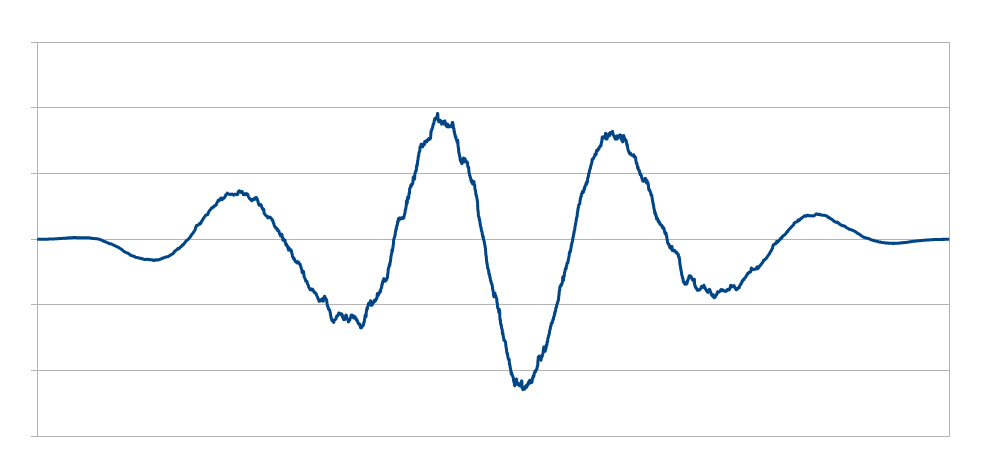
\includegraphics[width=\textwidth]{windowed_buffer}
	\caption{What the signal looks like after applying the Hann window function. The buffer has been rotated so that the point of discontinuity is at $x=0$. Since the Hann window function is 0 at the first and the last point we get a continuous signal suitable for the frequency analysis.}
	\label{fig:Hann window}
\end{figure}

\section{Frequency analysis}
\index{Fast Fourier Transformation}
The next step of the audio processing is the \gls{FFT}. 
The \gls{FFT} is a method to transform a signal from time domain to frequency domain. The result is a list of complex numbers that represent the amplitude and phase of each frequency. 
We used the {\tt KissFFT} library (see \ref{sec:KissFFT}) for the calculation. 
Because the \gls{FFT} is meant to be used on stationary signals while we are dealing with a continuous signal, we split up the input into slices, each a few milliseconds in length and apply a window function to them. 
Samples from the audio device are written into a ring buffer and once a certain amount of samples have been written the \gls{FFT} is applied to them. The frequency spectra overlap each other to get a higher time resolution while maintaining a high frequency resolution. 

\section{Removing noise}
Most noise in audio signals appears as an always prevalent amplitude on certain frequencies. To remove it, the minimum amplitude that has been measured on a frequency so far is subtracted from the measurement. 

To achieve this, the program keeps a list with the minimum amplitudes for multiple frequency ranges.

\section{Automatic equalizer}
Additionally to the difference in overall sensitivity, cheap pick-ups and microphones also show different sensitivity for different frequencies. For better note detection an equalizer is applied to the signal. 

An equalizer amplifies or tones down individual frequencies. Since the spectrum of guitars spread rather evenly over the whole frequency range the sensitivity can be measured by finding the maximum amplitude that is measured on a frequency range so far. 

Additionally to the list of minima that is used for the noise removal, the program also keeps a list of the maximum amplitude for multiple frequency ranges. The equalized amplitude for a frequency is calculated as 
$$a'(F, t) = \frac{a(F, t) - min(F)}{max(F) - min(F)}$$
where $a(F, t)$ is the amplitude of frequency $F$ at time $t$ and $min(F)$ and $max(F)$ are the minimum and maximum amplitudes measured in the range $F$ lies in.

\section{Applying the scoring function}
Every natural sound consists of a fundamental frequency and a set of overtones whose frequencies are decimal multiples of the fundamental frequency (see figure \ref{fig:Bass spectrum}). Since the overtones can (and the first one always will) fall on the frequencies of other pitch values they have to be filtered from the signal. We use a scoring function to determine how likely a given frequency is a note.

\begin{figure}
	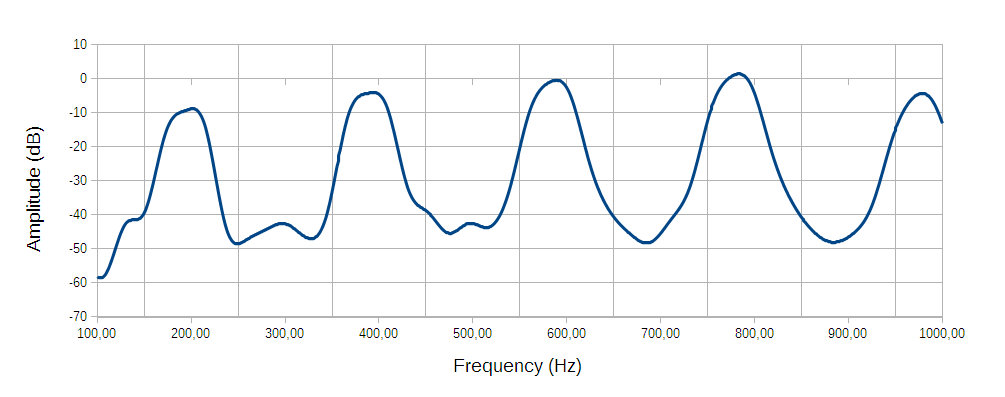
\includegraphics[width=\textwidth]{bass_spectrum}
	\caption{The frequency spectrum of a bass guitar playing the note G3. Notice the fundamental frequency at about 200 Hz and the overtones at multiples of that frequency.}
	\label{fig:Bass spectrum}
\end{figure}

To remove overtones and also increase frequency resolution we apply a scoring function that is defined in such a way that frequencies with overtones but no undertones get the highest score. 
The score for a pitch is defined as
$$ score(x) = \sum_{i = 1}^{I}\frac{F(x * i)}{\sqrt{i}} - \sum_{i = 2}^{I}\frac{F(x / i)}{\sqrt{i}} $$
where $x$ is the current frequency, $F(x)$ is the amplitude of frequency $x$ and $I$ is the number of overtones to look for.

Possible notes will show up as local maxima in the resulting function.
Because of accuracy issues and noise it often also detects notes near the actual note. To account for this, we only consider frequencies that are a maximum  within a certain radius. For a radius we chose one semi-tone because accords with notes that close together (a {\em major second}) are very unusual in modern music. 

\section{Automatic thresholds}
After potential pitches have been determined, they are compared to a threshold. The optimal value for this varies between different instruments and audio hardware. Multiple algorithms to find the best threshold have been tried out. These are described here.

\subsection{Finding the two most distant clusters}
The most basic algorithm to find a threshold is implemented in the class {\tt AutoThreshold}. Basically, it consists of a single function {\tt bool is(int value)}, which compares a value to the threshold and adjusts the threshold. 

For reasons of efficiency, the threshold is not updated every time a new value is compared but only after a call to the function {\tt update()}.

The algorithm underlies the idea that the distribution of measurements creates two cluster points. By counting how often each value has been compared it tries to find these clusters and then determines the threshold. 

To find the optimal threshold the algorithm splits up the set of measured amplitudes in such a way that the emerging subsets' averages are as far apart as possible. This is achieved by iterating over all possible thresholds.

The ideal threshold is the one for which the following expression reaches its maximum 
$$ \frac{\sum_{i = t}^{N - 1}(i * P(i))}{N - t} - \frac{\sum_{i = 0}^{t - 1}(i * P(i))}{t} $$
where $t$ is the index of the first range that lies just above the threshold, $N$ is the number of ranges and $P(i)$ is the number of measurements that fall into the range at index $i$.

Since the ratio between silence and playing can vary the algorithm should still work if one of the two clusters is much higher. This is where this method fails. If the clusters are not of similar size the distance between them can be increased by moving the threshold beyond the smaller.

\subsection{Finding the two narrowest clusters}
This algorithm underlies the same principles the previous one does but instead of trying to have the two clusters as distant as possible they should be as narrow as possible. Therefore we calculate the variance of both subsets and try to minimize their sum.

First we calculate the average values of both sets with 
$$ \mu_{0} = \frac{\sum_{i = 0}^{t - 1}i * P(i)}{t} $$
$$ \mu_{1} = \frac{\sum_{i = t}^{N - 1}i * P(i)}{N - t} $$
and then the sum of the variances of both subsets as
$$ \sum_{i = 0}^{t - 1}P(i) * (i - \mu_{0})^{2} + \sum_{i = t}^{N - 1}P(i) * (i - \mu_{1})^{2} $$
where $t$ is the index of the first range that lies just above the threshold, $N$ is the number of ranges and $P(i)$ is the number of measurements that fell into the range at index $i$.

This approach is only useful when the notes have similar volume since else the cluster for the upper cluster spread to much. Additionally, this solution is rather slow even on modern computers.

\subsection{Considering the number of notes we are looking for}
This is a very different approach as it does not rely on statistics about the signal but instead considers how many notes an instrument can play at once. Most guitars have 4 to 6 strings and therefore can play only that many notes at once. Additionally we assume that all simultaneous notes have about the same volume. 

After the maxima in the scoring function have been found we look for the highest score and consider every other maxima that is not much quieter than that as a note. If the number of notes found is bigger than 6 we consider the signal noise as it can not come from a guitar.

\chapter{Audio output \textsuperscript{Neumayer}}
\label{chap:Audio output}

One of the most important aspects of any audio-related project is how well the software 
performs real-time audio output operations. Low latency is especially critical 
when users expect an instant response of the application. 

\section{Differences between platforms}

While Qt allows multi-platform development of natively compiled applications, 
there are still cases where differences between supported platforms have to be 
taken into account. It was decided that a timer-based approach was inappropriate 
and therefore, a thread-based solution would have to be used. The problem with basing audio output on a periodic timer is that, while it worked perfectly on Linux, Qt on Windows 
didn't provide timers with sufficiently high accuracy. This is due to a deficiency in the Windows audio stack which Qt's timers are based on.

\section{Audio output using Qt}

The Qt framework provides facilities to access audio hardware in an abstract way. 
In the case of Beat The Score the used classes are {\tt QAudioFormat}, {\tt QAudioDeviceInfo} and {\tt QAudioOutput}.

\subsection{QAudioFormat}

{\tt QAudioFormat} is used to tell the audio hardware information about the sound data that will be 
written to it.
\\

\begin{lstlisting}
QAudioFormat format;
format.setSampleSize(16);
format.setSampleRate(44100);
format.setChannelCount(1);
format.setCodec("audio/pcm");
format.setByteOrder(QAudioFormat::LittleEndian);
format.setSampleType(QAudioFormat::SignedInt);
\end{lstlisting}

Audio data is made of individual samples. The sample size defines how many bits a single 
sample has. The sample rate describes how many samples audio data can have within the 
time span of one second. Channel count refers to the number of concurrent channels the 
audio data has. In Beat The Score only audio data with a single channel is used. 
\\
The codec tells the audio device which format the to-be-expected audio data has. 
According to the Qt documentation \footnote{\label{foot:1}http://qt-project.org/doc/qt-5/qaudiodeviceinfo.html\#supportedCodecs}, 
'All platform and plugin implementations should provide support for: "audio/pcm"'.
\\
Beat The Score uses audio files in the RIFF WAVE format, which is an uncompressed, 
raw audio format with meta data about its sample rate, bits per sample, et cetera. 
According to the RIFF WAVE specification \footnote{\label{foot:2}https://ccrma.stanford.edu/courses/422/projects/WaveFormat/} samples are expected to be both little-endian and, in the case of 16-bit samples, signed.

\subsection{QAudioDeviceInfo}

In order to access the audio device with a supported audio format Qt provides 
functionality to check if the audio hardware actually supports the declared format.

\begin{lstlisting}
QAudioDeviceInfo info(QAudioDeviceInfo::defaultOutputDevice());
if (!info.isFormatSupported(format)) {
    cout << "format sadly unsupported, trying to find nearest format" << endl;
    format = info.nearestFormat(format);
}
\end{lstlisting}

The static public method {\tt QAudioDeviceInfo::defaultOutputDevice()} is a factory method that, 
depending on the targeted platform, returns an object which represents the audio hardware 
to output sound. The source code of Qt that is referred to in this section is released 
as version 5.2.1 of Qt. \footnote{\label{foot:3}https://qt.gitorious.org/qt/qtmultimedia/source/\\9a16423610405c0329fe40235313212946f08b05:src/multimedia/audio}
On systems where the ALSA audio architecture is used (Linux and Android), 
the first audio device that can be found on the system is used, 
according to the source code of qaudiodeviceinfo\_alsa\_p.cpp. 
On Windows (qaudiodeviceinfo\_win32\_p.cpp) Qt selects the default 
audio device based on the WAVE\_MAPPER device identifier.
\\
The output device is provided to the constructor of {\tt QAudioDeviceInfo} which allows 
information about the device to be gathered. This is used to decide whether the 
device actually supports the desired audio format. In case the requested format is 
not supported, the application tries to find a format that is similar to the requested 
format using the {\tt nearestFormat()} method of {\tt QAudioDeviceInfo}. This method compares 
the formats that are supported by the device with the provided format and returns the 
most similar format, based on codec, byte order, sample type, sample size, channel count, 
and sample rate.

\subsection{QAudioOutput}

After an audio device with a supported format has been selected it is possible to create an 
object of type {\tt QAudioOutput} to send sample data to the audio hardware. 
According to the Qt documentation \footnote{\label{foot:5}http://qt-project.org/doc/qt-5/audiooverview.html}, {\tt QAudioOutput} provides two modes to accomplish this: 

\begin{description}
\item [Pull mode] The {\tt start()} method of a {\tt QAudioOutput} object can be given a pointer to {\tt QIODevice} object as a parameter. In this case the {\tt QIODevice} contains a buffer with mixed audio samples. Doing this will make the {\tt QAudioOutput} decide for itself when to pull audio samples from the {\tt QIODevice}. The decision when to pull samples is based on how many samples can be sent to the sound card for one period. The duration of a period can vary during runtime. \hfill \\
\item [Push mode] When the {\tt start()} method of a {\tt QAudioOutput} object is called without a parameter, it returns a pointer to a {\tt QIODevice} object. The application has to write audio samples to this {\tt QIODevice} by itself periodically. This approach is more appropriate for real-time audio as the fluctuating nature of the pull mode does not guarantee low latency sound output. \hfill \\
\end{description}

It was decided to use the push mode in Beat The Score as it is more appropriate for real-time audio use cases.

\section{Pitching audio samples}

To easily and quickly pitch audio samples the application uses the SoundTouch library by 
Olli Parviainen \footnote{\label{foot:5}http://www.surina.net/soundtouch}. SoundTouch provides an implementation 
of the Synchronous-Overlap-Add algorithm. 
\\ \\
To quote an article of Olli Parviainen \cite{soundtouch1}: 
\linebreak
\begin{quote}
SOLA, being short-hand for Synchronous-OverLap-Add, works by cutting the sound data into 
shortish sequences between tens to hundreds milliseconds each, and then joining these 
sequences back together with a suitable amount of sound data either skipped or partially 
repeated in between these sequences, to achieve a shorter or longer playback time than originally.
\end{quote}

For details on how to use the SoundTouch API please refer to section \ref{sec:SoundTouch} for more information.
\\
Beat The Score ships with samples for guitars, pianos and drums in the RIFF WAVE format. 
The file name of these samples corresponds to its MIDI note number as defined 
by the MIDI specification. 

\begin{center}
\begin{tabular}{ | l | l | }
  \hline
  MIDI note number & note \\ \hline
  .. & .. \\ \hline
  48 & C \\ \hline
  49 & C\# \\ \hline
  50 & D \\ \hline
  51 & D\# \\ \hline
  52 & E \\ \hline
  \hline
\end{tabular}
\end{center}

For each of the instruments there are only sample files of the note C in different octaves. 
When the application starts, it reads these existing samples from the file system and 
pitches missing semitone steps to get valid samples for each octave in a loop until 
there is a sample for every possible MIDI note number.
\\ \\
Internally, the application creates a vector of {\tt NoteSample}s where a 
{\tt NoteSample} is a C++ data structure.
\\ \\ \\ \\ \\ \\ \\ \\ 
\begin{lstlisting}
struct NoteSample {
    NoteSample()
    {
        buffer = NULL;
    }
    ~NoteSample()
    {
        if (buffer != NULL)
            delete buffer;
    }

    char * buffer;
    int bufferSize;
};

vector<shared_ptr<NoteSample>> notes; // index is the note number as specified in the MIDI spec
\end{lstlisting}

A {\tt NoteSample} represents exactly one note. What MIDI note number a {\tt NoteSample} 
relates to is identified by the vectors index. The {\tt char *} inside the 
struct {\tt NoteSample} points to an address in memory where its audio samples are 
stored and the buffer size defines the buffers size in memory. As a result 
there are 128 {\tt NoteSample}s in the vector for the MIDI note numbers from 0 to 127.

\section{Audio mixing}

An audio mixer is needed to play multiple notes at the same time. 
This is implemented in the C++ class called {\tt AudioBuffer}. 
The header file of {\tt AudioBuffer} looks as follows:
\\
\begin{lstlisting}
class AudioBuffer
{

private:
    vector<shared_ptr<NoteSample>> noteBuffers;
    vector<int> notePositions;
    QMutex mutex;

public:
    AudioBuffer(qint64 maxSize);
    ~AudioBuffer();
    qint64 readData(char * mixedBuffer, qint64 size);
    void writeData(shared_ptr<NoteSample> note);
    void writeData(shared_ptr<NoteSample> note, int offset);
    void clear();
};
\end{lstlisting}

The vector {\tt noteBuffers} contains shared pointers to {\tt NoteSample}s and \\ 
{\tt notePosition} contains the information on how many samples of the {\tt NoteSample}s 
buffer have been read. 
The {\tt QMutex} object is provided by the Qt framework and used to handle access to the {\tt NoteSample}s, so that {\tt NoteSample}s cannot be added to the mixer while audio is being mixed at the same time.
\\
The method {\tt readData} is used to mix the buffers of each {\tt NoteSample} together. \\
\begin{lstlisting}
qint64 AudioBuffer::readData(char * mixedBuffer, qint64 size)
{
    QMutexLocker(&this->mutex);
    // Let's only add up samples that overlap at a single point in time.
    // Also, do mixing in relation to the longest buffer in the vector.
    int longestSample = 0;

    for(int i = 0; i < noteBuffers.size(); i++) {
        if(noteBuffers[i]->bufferSize > longestSample) {
            longestSample = noteBuffers[i]->bufferSize < size ?
                        noteBuffers[i]->bufferSize : size;
        }
    }

    // Step through every single point in "time" and mix samples that overlap
    for(int i = 0; i < longestSample; i+=2) {
        short mixedValue = 0;
        int mixBufferCount = 0; // How many buffers can be mixed at this point in time?
        for(int j = 0; j < noteBuffers.size(); j++) {
            shared_ptr<NoteSample> sample = noteBuffers[j];
            if(sample != NULL && notePositions[j] >= 0 &&
                    (sample->bufferSize - notePositions[j]) > 0) {
                mixBufferCount++;
            }
        }

        for(int j = 0; j < noteBuffers.size() && mixBufferCount > 0; j++) {
            shared_ptr<NoteSample> sample = noteBuffers[j];
            if(sample != NULL && notePositions[j] > 0) {

                // Can this part of the sample be mixed?
                int length = (sample->bufferSize - notePositions[j]) > size ?
                        size : (sample->bufferSize - notePositions[j]);

                if(length > 0) {
                    short tmpVal = 0;
                    memcpy(&tmpVal, &(sample->buffer[notePositions[j]]), 2);
                    tmpVal = tmpVal / mixBufferCount;
                    mixedValue += tmpVal;
                }
            }

            notePositions[j] += 2;
        }

        memcpy(&mixedBuffer[i], &mixedValue, 2);
    }

    // Remove notes from the vector if they have been mixed completely
    for(int i = noteBuffers.size()-1; i >= 0; i--) {
        shared_ptr<NoteSample> sample = noteBuffers[i];
        if(sample->bufferSize < notePositions[i]) {
            noteBuffers.erase(noteBuffers.begin()+i);
            notePositions.erase(notePositions.begin()+i);
        }
    }

    // Append silence in case there is still some room for values
    if(longestSample < size) {
        memset(mixedBuffer+longestSample, 0, size-longestSample);
    }

    return size;
}
\end{lstlisting}

The parameter {\tt size} describes how many "parts" of each individual buffer have to be mixed. 
These parts are generally referred to as samples. After the desired samples have been read 
from a buffer the corresponding position is incremented by the value of the {\tt size} parameter. 
When mixing, the numerical values of concurrent samples are added together and divided by 
the number of concurrent {\tt NoteSample}s. The resulting value gets copied into the provided 
character pointer called {\tt mixedBuffer}. If the position of a {\tt NoteSample} exceeds its 
buffer size the {\tt NoteSample} and its position are removed from their respective vectors. 
After the process of mixing is done the method returns the provided size.
\\
The method {\tt writeData} is used to put {\tt NoteSample}s into the vector and 
initializing its position, either by initializing the {\tt position} with 0 
or by an optionally provided offset. The optional {\tt offset} paramenter describes by how many samples 
mixing of this specific {\tt NoteSample} has to be delayed. A position of 0 indicates that the 
{\tt NoteSample}s buffer has to be mixed as soon as the {\tt readData()} method is called, 
a position of negative value delays the mixing of the specific {\tt NoteSample} 
into the future and a position of positive value would cause {\tt readData()} to skip samples.

\section{Output of instruments}

Catching MIDI signals and turning them into something that the application can 
understand is done by the {\tt MidiInput} class. Depending on the platform the 
application runs on, this class uses either RtMidi on Windows and Linux or libusb on 
Android to read the MIDI data and putting its values in a {\tt Note} object. 

\section{Output of background music}

Background music is considered to be every track of the music except the selected input 
track. These tracks are looped through in a separate background thread inside the {\tt NoteOutput}  
object. Looping through the tracks is done periodically, just like the actual audio 
output itself, every 20 milliseconds. This background thread runs synchronously with the 
game's internal clock to not mix samples into the master buffer when the game pauses or 
when the user is in the main menu. 
\include{automatischesoftwareverteilung}
\chapter{Sales platform \textsuperscript{Neumayer}}

Parts of the diploma project were the implementation of a web site to sell the application and a way to handle licenses to use the application. The sales platform is split into two parts:

\begin{description}
\item [The frontend:] provides the web site to purchase the license from and a RESTful API that can be accessed using HTTP requests. \hfill \\
\item [The backend:] generates and stores user licenses in a local SQLite database and validates them. \hfill \\
\end{description}

The backend and frontend run on a Linux-based server and communicate through an IPC mechanism called D-Bus.

\section{D-Bus}

Note: The following description is based on information from the FreeDesktop wiki.\cite{dbus1}
\\
D-Bus, short for "Desktop Bus", is an inter-process-communication mechanism used to allow 
processes to call functions of other processes in a secure, predictable, and 
standardized manner. Although it is mostly used in applications with graphical user interfaces 
and desktop environments on Unix-like platforms, D-Bus does not have a functional dependency 
on graphical environments. Implementations of D-Bus are available for Linux, BSD and Windows, 
among other operating systems.
\\
Some of the most important features of D-Bus related to this project which lead to the conclusion that choosing D-Bus as the only viable IPC mechanism, are:
\begin{itemize}
\item {Communication between processes without the need of the network stack of the operating system kernel: the backend doesn't have to listen on a network-based socket. Having two processes on the same machine exchanging information over the network stack of the operating system would unavoidably add overhead to the exchanged messages.}
\item {Influenced by object-oriented programming languages: Methods which are exposed via D-Bus are identifiable by a globally unique name space, which is akin to what object-oriented programming languages provide. This provides a familiar development environment and eases the process of finding errors.}
\item {The ability to introspect exposed methods: it is possible to browse through all exposed methods on the message bus at run time, checking their method names, parameters and return types. This makes the efforts of debugging the communication less complicated.}
\item {Access control via policy handling: Access to the exposed methods can optionally be granted to specific applications only, for example by which user account started the client process. This feature adds an extra layer of security and ensures that information does not leak into unprivileged processes.}
\item {On-demand activation: The server process can be started automatically by the D-Bus daemon as soon as a client process tries to access the exposed methods. This can be accomplished by an XML-based configuration file which makes the executable path of the server process and its exposed methods known to the bus daemon.}
\end{itemize}

\section{Frontend}
To serve web pages to potential customers and provide a REST-ful API, a frontend server runs on the TCP port 80. This server is implemented in the Python programming language and it uses the programming library Bottle for its templating system. Using this templating system it is possible to stitch parts of the website together at runtime for each seperate HTTP request.

\section{Backend}
The backend is a background daemon program which is implemented in \cpp. To store data about customers and their licenses the daemon writes to a SQLite database. Licenses are generated for uses through asymmetrical encryption using APIs provided by OpenSSL.

\section{Separation of privileges}
The frontend and the backend are separated from each other to provide a more secure architecture. As the public way to access the data on the database is through the frontend (via HTTP requests), it is critical to avoid vulnerabilities which could be triggered by third-parties. 
\\
Process-level separation already provides some security as the sales platform is split into two parts and operating systems usually have the required mechanisms built into them to not allow one process to read memory of another process. To further secure the architecture, both processes run as separate users and each user only has access to its own contained directory.

\section{Communication between frontend and backend}
To allow the frontend to return license data to the user it needs a well-defined interface to get access to the data. As mentioned before, the backend provides an interface which can be accessed through the D-Bus IPC mechanism. Only the user of the frontend process has access to this interface as provided by the specific D-Bus policy file. The D-Bus policy file looks like this:

\begin{lstlisting}
<!DOCTYPE busconfig PUBLIC
 "-//freedesktop//DTD D-BUS Bus Configuration 1.0//EN"
 "http://www.freedesktop.org/standards/dbus/1.0/busconfig.dtd">
 
<!-- This file has to be copied to /etc/dbus-1/system.d/ -->
<busconfig>
        <policy user="btsbackend">
                <allow own="at.beatthescore.license"/>
        </policy>
        <policy user="btsfrontend">
		        <allow send_destination="at.beatthescore.license"/>
        </policy>
        <policy context="default">
                <deny own="at.beatthescore.license"/>
        <deny send_destination="at.beatthescore.license"/>
        </policy>
</busconfig>
\end{lstlisting}

Policies have a higher priority the higher it is placed inside the {\tt busconfig} element. The {\tt policy} element contains information about what can be allowed and what has to be denied. Attributes like {\tt user}, {\tt group}, and {\tt context} define which users or groups of users the specific policies apply to. A policy with a {\tt context} value of {\tt "default"} applies to every user.
\\
Since access to the interface for every user is denied the policy configuration makes sure to "punch holes" to allowed users before access gets locked down completely. This is achieved through the two topmost {\tt policy} elements. In this example the {\tt "at.beatthescore.license"} defines the name space on the communication bus. The two topmost policies specify:
\begin{enumerate}
\item{only the user of the backend daemon should be allowed to own the name space for exposing methods on the bus}
\item{only the frontend's user should be allowed to access methods on the bus in the same name space}
\end{enumerate}

Also, by default the D-Bus daemon provides two main buses:
\begin{description}
\item[System bus:] \hfill \\ The system bus allows processes to access methods of other processes which are not running in the session.
\item[Session bus:] \hfill \\ This bus allows processes which are owned by a specific user session to communicate.
\end{description}

\section{Customer login}
Customers create user accounts by logging into the site using Mozilla Persona. Mozilla Persona  \footnote{\label{foot:2}http://persona.org} is an implementation of the BrowserID protocol and allows us to create a login system without having to save login data persistently on the server. Through the use of Persona we are confident that passwords of users won't get compromised in case of a security breach on the server. The email address of the customer is used as the only identifier globally in the database.

The login happens by clicking the respective button on the website.
\\
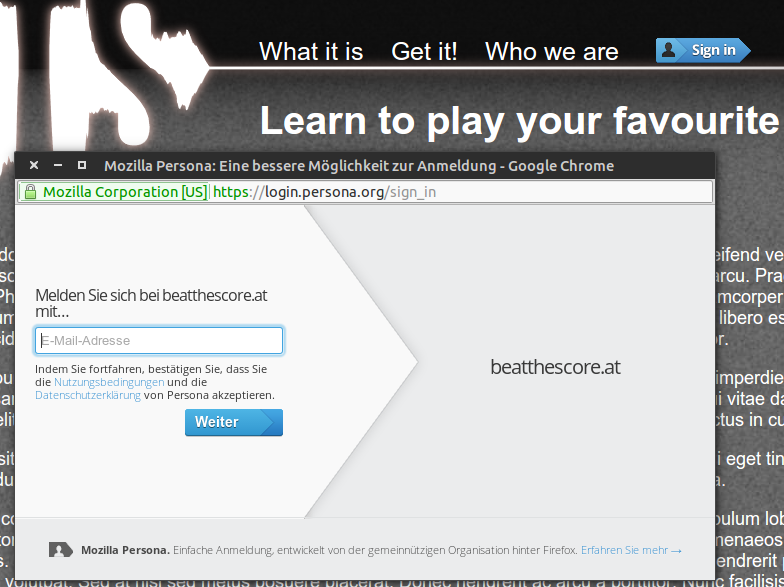
\includegraphics[width=1.0\textwidth]{bts_login}
\\
When the customer enters his email address he can be authorized to use the website using one of the 3 following ways:

\begin{description}
\item [Authorization using identity provider:] If the email provider has implemented an identity provider the authorization will continue seamlessly. \hfill \\
\item [Authorization using OpenID:] Persona can authorize the user on the website using OpenID in case the provider does not natively implement an identity provider. Of course this only works if the email provider is also an OpenID provider. \hfill \\
\item [Authorization using email:] As a fall back, in case none of the mentioned authorization methods can be used, the customer will get an email sent to his email address. This email would contain a link through which the used can authorize himself manually. \hfill \\
\end{description}

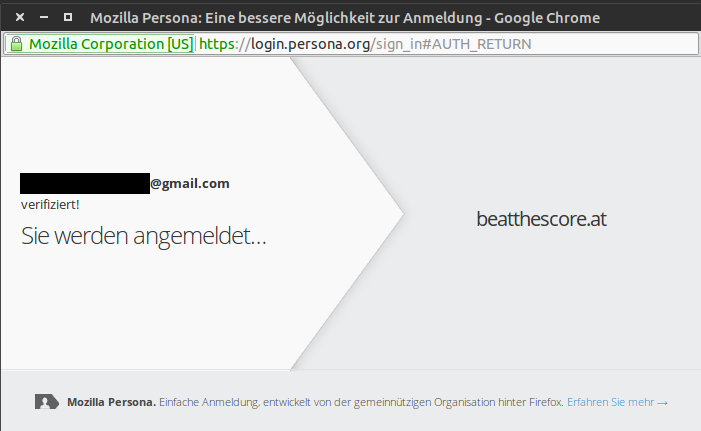
\includegraphics[width=1.0\textwidth]{bts_authorized}

If the authorization is successful the browser will send an HTTP POST request to {\tt beatthescore.at/verify} where we can further validate assertion data with a verification endpoint. In the case of the Beat The Score website we use Mozilla's own verification endpoint (verifier.login.persona.org). Verification is done in the frontend using Mozilla's browserid Python library.
\begin{lstlisting}
@route('/verify', method='POST')
def verify():
    body = request.POST
    assertion = body['assertion']
    print(assertion)
    data = browserid.verify(assertion, ASSERTION_URL)
    licenseManager.InsertUser(data['email'])
    sess = request.environ.get('beaker.session')
    print(sess)
    sess['email'] = data['email']
    return simplejson.dumps({ 'email' : data['email'] })
\end{lstlisting}

\begin{enumerate}
\item In case the verification fails the server will send back an error to the customers web browser and authorization fails.
\item If the verification is done successfully the email address will get sent to the backend process using {\tt licenseManager.InsertUser(data['email'])}. 
\item In case the backend is unable to parse the provided string the email address will not be inserted into the SQLite database and the authorization fails.
\item If the backend process successfully inserts the customers email address into the database a session cookie will be set to indicate a successful authorization to the customers web browser. 
\end{enumerate}

\section{Selling licenses through PayPal}
To further automate the selling of user licenses to customers we decided to use PayPal. PayPal is used by millions of people around the globe and provides several mechanisms for payment automation. All possible ways to integrate PayPal can be found on their developer portal. \footnote{\label{foot:3}https://developer.paypal.com/}
\\
Some of the options which were discussed while designing the payment workflow were:

\begin{description}
\item [PayPal Mobile SDK] Developers can embed views into their applications to allow users to purchase a license. This mechanism can not apply to Beat The Score as there is no SDK for Qt applications. Also this would require releasing a free version of the software package. \hfill \\
\item [PayPal Instant Payment Notification] Using IPN a merchant can receive an HTTP POST request to a URL of choice as soon as a customer completes a payment transaction to the merchants email address. The merchants web server can then send a request to a PayPal server to check if the POST request actually originated from PayPal and whether the received payment transaction is valid or not. The downside is that this approach is asynchronous by design and one of the design goals was to have the whole purchasing process happen in a single browser window. Also, this fits better into use cases where the customer receives the requested goods via email. \hfill \\
\item [PayPal Express Checkout] Express Checkout provides a way to integrate PayPal into the web sites workflow where a successful purchase would immediately result in showing the licenses activation code, all in the same browser window. This activation code could then be entered into the application's window. \hfill \\
\end{description}

\section{License generation}
As soon as the payment transaction is validated and completed, a license file should be generated for the user. This license file is generated in the backend process and inserted into the database afterwards. The license file is generated by using RSA for asymmetrical encryption and SHA256 hashes.

\begin{enumerate}
\item Concatenate the buyers email address and the date of purchase into a string.
\item Generate a SHA256 hash of the concatenated string and represent it in hexadecimal numbers.
\item Concatenate the original string with a newline character and the hexadecimal hash.
\item Encrypt the result with a private RSA key.
\item Apply Base 64 encoding to the result of the encryption.
\end{enumerate}

The Base 64 encoded blob is then inserted into the database. Afterwards, an activation code is generated that is only valid for 5 minutes. Doing this ensures us that the same activation code cannot be used more than once over a long period of time.

\section{Entering the activation code}
As soon as an activation code is generated it can be entered into the application window, together with the customers email address that was used to authorize the user using Mozilla Persona.
\\
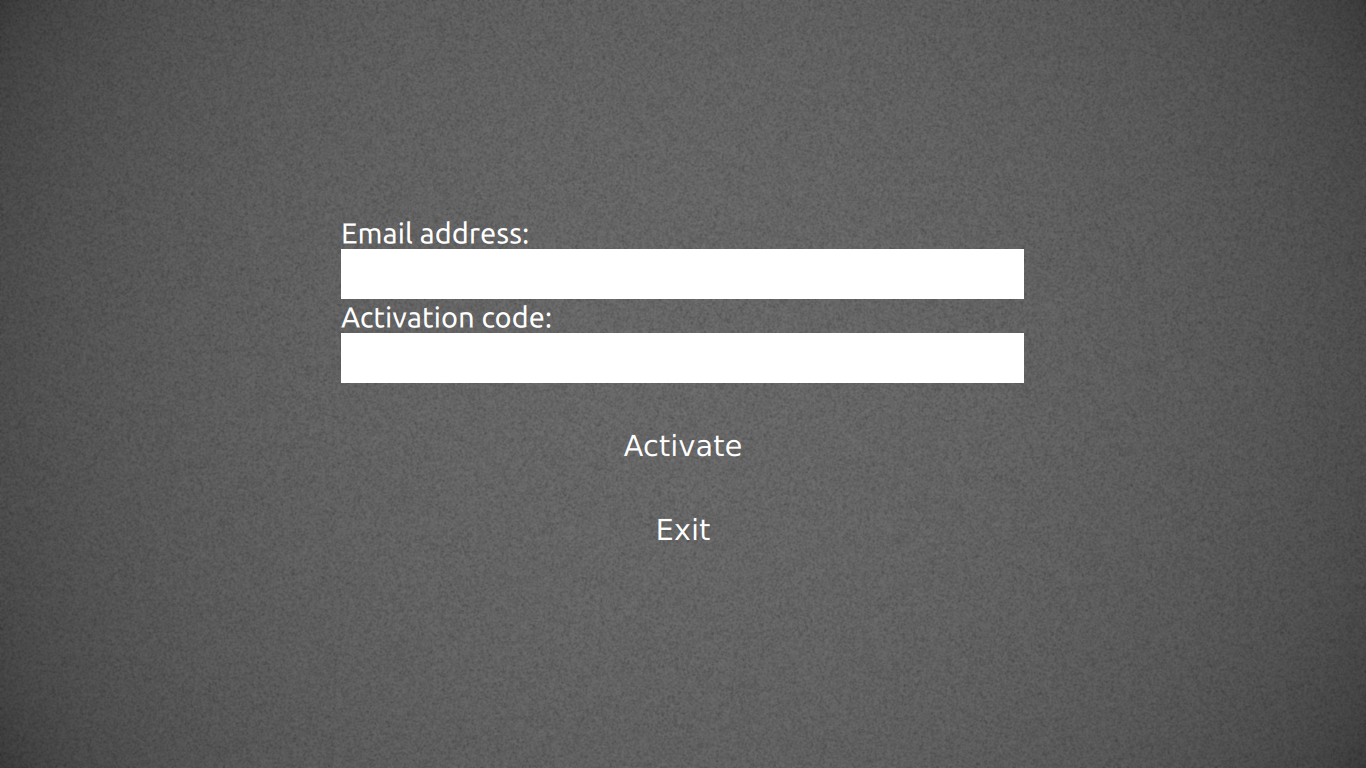
\includegraphics[width=1.0\textwidth]{license_enter}
\\
\begin{enumerate}
\item The application will try to validate the activation code and send an HTTP POST request to the frontend server.
\item The frontend server will pass the activation code to the backend process to check if the activation code is valid, if the code is related to an existing license and if the license actually belongs to the entered email address.
\item If all of those checks pass, the backend will read the license from the database and pass it to the frontend.
\item The frontend will in turn send that data back to the application. 
\item The application then saves the license file locally on the file system and validate the license. If the license validation succeeds the user can start using Beat The Score.
\end{enumerate}
\chapter[User Interface Implementation \textsuperscript{Novotny}]{User Interface Implementation}
\label{chap:UI}
The implementation of the user interface is based on QML. \\
This chapter explains how the user interface was constructed. QML and the components that have been used for building the user interface are explained in chapter 3.
\paragraph{Organisation of the Chapter} The first part of this chapter gives an overview of the initialization process required before the first menu page is loaded. The second part explains the architecture of the user interface. The next section explains how the different methods of menu navigation have been implemented. The third section deals with the components used throughout the menu pages. At the end of the chapter a number of sections deal with side processes (such as storing and retrieving user data) that are triggered by the user interface.
\section{Initialization and Data Supply}
An {\tt ApplicationViewer} is responsible for displaying the user interface.
In order to allow communication between the \cpp and the QML side of the application two context properties are passed to the {\tt ApplicationViewer} object:

\begin{itemize}
	\item{{\tt licenseManager}}
	\item{{\tt game}}
\end{itemize}

The {\tt game} property points to the {\tt MainGame} object instantiated in the main method (refer to \ref{chap:Design}) for an explanation of the role of this object). This property is the most important communication interface between the user interface and the application logic.
Its main responsibilites include:
\begin {itemize}
	\item {Supplying data such as {\tt Scores}, {\tt Tracks} and {\tt Devices}.}
	\item {Controlling the flow of the application by triggering the start of a song and maintaining state information (refer to the chapter \textit{Design} for a more detailed explanation).}
\end {itemize}

A {\tt SoundNavigationHandler} object responsible for passing sound-based navigation instructions which has a pointer to the {\tt ApplicationViewer} object is created right after the user interface is initialized. The responsibilites of this object are discussed in detail at a later point.

\section {Menu Structure}
When the application starts a QML component called {\tt DisplayLoader} is loaded. 
Its responsibilites include 
\begin {itemize}
	\item {Dynamically loading the menu pages. This is accomplished using the {\tt Loader Element}. When {\tt DisplayLoader} is first created the Main Menu is loaded. Thereafter, the individual menus are responsible for resetting the source of the item to be displayed in the DisplayLoader.
	\begin{lstlisting}
		Loader {
			id: loader
			anchors.fill: parent
		}
	\end{lstlisting}
	The menus may change the source of the loader as follows.
	\begin{lstlisting}
		CustomButton {
			id: startButton
			buttonText: "Start"
				
			onClicked: {
			     	loader.source = "GameSettings.qml"
			 }
		}
	\end{lstlisting}
	}
	\item {
	Supplying global parameters concerning the environment and the appearance of the application. These include:
	\begin {itemize}
		\item{appearance parameters such as font, font-size and color}
		\item{environment parameters such as name and location of the database, API links, ...}
		\item{layout parameters such as insets and margins}
	\end {itemize}
	}
\end {itemize}
\section{Navigation}
As explained in chapter \ref{chap:UserInteractionConcept} the application supports three user interaction concepts.
\begin{itemize}
	\item {Mouse-Based Navigation}
	\item {Sound-Based Navigation}
	\item {Keyboard-Based Navigation}
\end{itemize}
\subsection{Sound-Based Navigation}
\label{sec:sound based navigation}
Commonly used navigation commands can be triggered by playing chords on a connected instruments. The following conditions need to be satisfied in order for a chord to be recognised:
\begin {itemize}
	\item {Chords consist of notes rather than pitches.}
	\item {Chords have to consist of three distinct notes.}
	\item {All notes of the chord need to be audible at the same time.}
	\item {Different inversions of the same chord are not distinguished. A \textit{D/F \#} chord is handled the same way a \textit{D} chord is handled.}
\end{itemize}
Playing a chord  while satifsying these conditions will be referred to as issuing a \textit{Sound-Based navigation instruction}.
\paragraph{Workflow}
This paragraph gives an overview of the process that is triggered in consequence of a single Sound-Based navigation instruction. The steps will be described in detail below.
\begin {enumerate}
	\item {The {\tt SoundNavigationHandler} recognizes a chord.}
	\item {It invokes the QML function {\tt handleCommand} defined in the {\tt DisplayLoader} element.}
	\item {The function emits a signal of the currently loaded menu page.}
	\item {This signal is received by the {\tt Chord} element of the current menu page. If a {\tt Chord} element finds out that its notes have been played it emits the signal {\tt played}.}
	\item {The signal is handled by the menu page.}
\end {enumerate}
\paragraph{Recognizing Chords}
Recognising chords is not necessary during game situations as single notes contained in the chord are evaluated separately. Chord recognition has been implemented for the sole purpose of allowing Sound-Based navigation. Chord recognition is done by the class {\tt SoundNavigationHandler}. {\tt SoundNavigationHandler} inherits {\tt QObject}. An object of this class is instantiated as soon as the {\tt ApplicationViewer} that displays the graphical user interface has been created. The {\tt ApplicationViewer} is the parent of the {\tt SoundNavigationHandler} object which means it will be destroyed automatically once the graphical user interface is destroyed. The class offers two slots:
\begin {itemize}
	\item{{\tt noteOn}}
	\item{{\tt noteOff}}
\end {itemize}
These slots are connected to the {\tt noteOn} and {\tt noteOff} signals of the {\tt Input} class while the menus are being used similarly to how these signals are connected to the {\tt Evaluator} class during game situations. \\
The object stores all notes that are currently being played (which means a {\tt NoteOn} but not corresponding {\tt NoteOff} event has been received) in a collection. As soon as there are three notes being played at the same time it considers the combination a chord. Note that only chords containing exactly three notes can be handled. 
The {\tt SoundNavigationHandler} object has a pointer to the {\tt ApplicationViewer} object. It can therefore invoke QML functions. This is used for communicating with the graphical user interface. 
\paragraph{Emitting the signal {\tt chordPlayed}}
The function {\tt handleCommand} that is defined in the {\tt DisplayLoader} element is invoked by the {\tt SoundNavigationHandler}. It receives a list containing the notes in the chord. It determines which menu page is currently loaded and then triggers the signal {\tt chordPlayed} of the active menu page. The signal is defined in the {\tt NavigatablePanel} element which is the root element of all menu pages.
\paragraph{Chord Element} The chord element is an invisible QML item. It stores an array of notes which make up the chord it represents. When a chord element is created it connects the parent's signal {\tt chordPlayed} to its function {\tt chordPlayed} which acts as a slot. This function decides whether or not the chord that was played is the chord represented by the element. It receives three midi pitch values. At this point midi pitch values are converted to musical notes represented by the letters A to G, using the \#-sign to indicate a pitch rise by a semi-tone. This is done using a modulo operation since musical notes repeat every twelve semitones. As a result the {\tt Chord} element discards the octave of the notes. This means that any inversion of a chord will be recognized.
\paragraph{Handling the {\tt Played} signal of a chord}
Six {\tt Chord} elements which are responsible for the most common user inputs are created in the {\tt NavigatablePanel} element. These include:
\begin {itemize}
	\item {Four chords corresponding to the arrow keys on the keyboard. If one of these chords is played the handling is done by the {\tt NavigatablePanel} element in a generic way that applies to all menu pages. This will be described in detail at a later point.}
	\item {A chord responsible for selecting the currently highlighted item of a {\tt SelectableListView} is defined by {\tt SelectableListView}}.
	\item {Additionally, two chords representing the following Commands are defined by {\tt NavigatablePanel}: 
		\begin {itemize}
			\item {instant confirmation of the settings made and proceeding to the next step}
			\item {discarding all settings and returning to the last step}
		\end {itemize} 
	A corresponding signal that can be handled by the active menu page is emitted when one of these chords is played.}
\end {itemize}
\subsection{Keyboard-Based Navigation}
When a key is pressed an event is delivered to the QML item that is currently focused. If the focused item does not accept the event it is passed up to its parent item until the event is handled or the root element has been reached. \\
Handling key events is done at different spots inside the user interface:
\begin {itemize}
	\item {
		Arrow key- and tab key events are handled by the root element of the active menu page. The root element of the menu pages is of type {\tt NavigatablePanel}.
	}
	\item {
		Return key events are handled by custom components such as {\tt CustomButton} and {\tt CustomCheckBox}. Using the return key when one of these components is focused has the same effect as clicking on the component.
	}
	\item {
		Space key events cause selection of the currently highlighted item of a {\tt SelectableListView}.
	}
\end {itemize}
The following code example shows how key events are handled by the {\tt CustomButton} element. 
\begin{lstlisting}
     // Keyboard Handling
     Keys.onPressed: {
         if (event.key === Qt.Key_Return && button.focus) {
             event.accepted = true;
             button.clicked();
         }
     }
\end{lstlisting}
Note that the event has to be accepted. Omitting this step will cause the event to be forwarded to the parent element of the button. Some buttons are used to change the source of a loader element which might cause the parent of the button to be destroyed which might lead to a segmentation fault.

\subsection{Generic Key Handling}
{\tt NavigatablePanel} handles a number of key events relevant to all inheriting menu pages:
\begin {itemize}
	\item {Arrow keys for moving inside a focused {\tt SelectableListView} or moving to the next component of the menu page. This is described in greater detail in the next section.}
	\item {The Enter key causes confirmation of all settings of the current dialog and proceeding to the next one. {\tt NavigatablePanel} emits the signal {\tt confirmed} which can be handled by the inheriting menu page.}
	\item {The Space key causes going back to the last dialog. The signal {\tt back} is emitted by {\tt NavigatablePanel} and may be handled by the inheriting menu page.}
\end {itemize}

\subsection{Generic Chord Handling}
{\tt NavigatablePanel} contains chord elements triggering certain actions: 
\begin {itemize}
	\item {one {\tt Chord} instance corresponding to each arrow key}
	\item {a {\tt Chord} instance corresponding to the enter key}
	\item {a {\tt Chord} instance corresponding to the space key}
\end {itemize}
The {\tt onPlayed} signals of these {\tt Chord} components are handled similarly to how the key events are handled.
\subsection{Focus Handling and Pre-Selection of List Items}
Focus Handling has been implemented in a generic way in the {\tt NavigatablePanel} element which is the root element of every menu page. \\
Every {\tt NavigatablePanel} element maintains an array called {\tt focusList} which contains all child elements that are part of the linear navigation flow. These elements are manually added to the element in the desired order when a menu page is created.
{\tt NavigatablePanel} provides the following functions.
\begin {itemize}
	\item {
		The function {\tt shiftFocus} triggers a focus shift by the passed amount. This means that the focus is given to another element of the {\tt focusList}. The parameter {\tt amount} can be positive (causing forward shifts) or negative (causing backward shifts). When the last element of the focus currently has the focus a positive shift will take the focus back to the beginning of the list. The opposite case is handled analogously.
	}
	\item {
		The function {\tt moveInActiveList} triggers a pre-selection shift in the {\tt SelectableListView} that currently has focus. It can be used similarly to {\tt shiftFocus}. When the last element of the list is selected a positive shift will not have any effect as the user might want to scroll to the end of the list quickly without being taken back to the beginning. The opposite case is handled analogously.
	}
\end {itemize}
The {\tt NavigatablePanel} has a property providing access to the currently focused component.

\subsection{Visual Feedback}
\subsubsection{Focused Component}
All custom components that can be focused ({\tt SelectableLisView}, {\tt CustomButton}, {\tt CustomCheckbox} ...) extend {\tt HighlightablePanel}.{}
\paragraph{\tt HighlightablePanel} consists of two {\tt Image} components:
\begin{itemize}
	\item {{\tt BackgroundImage}}
	\item {{\tt SourceImage}}
\end{itemize}
The {\tt source} property of these components can be accessed via the {\tt imageSource} and {\tt highlightSource} property aliases of {\tt HighlightablePanel}. The inheriting component is responsible for setting the visibility of the images.
\section {Components}
\subsection{Standard Components, Reasons for Implementing Custom Components}
QML provides a number of basic components which serve as building blocks for custom components rather than functional parts of the user interface.
This type of components include:
\begin{itemize}
	\item{{\tt Item}}
	\item{{\tt Rectangle}}
	\item{{\tt MouseArea}}
\end{itemize}
and many others. These components are treated in Chapter 3.

The package {\tt QtQuick Controls} offers a range of controls commonly used in applications. The appearance of these components is specific to the platform and therefore provides a native look and feel. However, there is no way to customize the appearance of the components while keeping the logic. All user controls were reimplemented to suit the look and feel of the application using only basic QML components as building blocks.

\subsection{NavigatablePanel}
The role of the {\tt NavigatablePanel} component is providing functionalities required by all menu pages. 
All menu pages inherit {\tt NavigatablePanel}. 

The responsibilites of {\tt NavigatablePanel} include:
\begin {itemize}
	\item {storing and retrieving data to/from the database,}
	\item {generic key event handling for key-based navigation,}
	\item {generic chord handling for sound-based navigation,}
	\item {generic focus handling.}
\end {itemize}

The functionalites of {\tt NavigatablePanel} are described in more detail in the corresponding sections.

\subsection{CustomButton}
The {\tt CustomButton} implements the function of a button while meeting the optical requirements of the application's user interface.  Primarily, this means to display different background images depending on the state of the button (default, hovered, highlighted), and to enlargen the button text when the button is highlighted.  The main building block for this custom component is the {\tt MouseArea} component provided by QML. Apart from reacting to mouse clicks the component reacts to keyboard events. 


\includegraphics[width=0.25\textwidth]{custom_button_a}

\includegraphics[width=0.25\textwidth]{custom_button_b}

{\tt CustomButton} offers the signal {\tt clicked} which can be emitted from within the component, which is done when the {\tt MouseArea} component detects a click or a key event is handled, or from without the component which is required for sound-based navigation (refer to the section on sound-based navigation for a in-depth explanation).

The component offers the following properties:
\begin {itemize}
	\item {{\tt buttonText}}
	\item {{\tt fontColor} sets the font color to be used for displaying the button text. If the property is not set explicitly the default font color defined in a global will be used.}
	\item {{\tt fontSize} sets the font size to be used for displaying the button text. If the property is not set explicitly the default font size defined in a global will be used.}
	\item {{\tt imageSource} sets the source of the default background image}
	\item {{\tt mouseHighlightSource} sets the source of the background image to be displayed while the component is hovered or focused.}
\end {itemize}

\subsection{CustomCheckBox}
The {\tt CustomCheckBox} implements the functionality of check box. 
{\tt CustomCheckBox} inherits {\tt HighlightableItem}.
The space key can be used for checking and unchecking the check box.


\includegraphics[width=0.5\textwidth]{custom_checkbox}

It provides the following properties:
\begin {itemize}
	\item {{\tt text} sets the text to be displayed next to the check box}
	\item {{\tt checked} indicates whether or not the check box is checked}
	\item {{\tt checkedSource}/{\tt uncheckedSource} set the source of the graphic to be displayed when check box is checked or unchecked}
\end {itemize}

\subsection{CustomSlider}
{\tt CustomSlider} implements the functionality of selecting a numeric value within a specified range while preventing the user from selecting illegal values. {\tt CustomSlider} components have a default value.

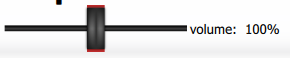
\includegraphics[width=0.5\textwidth]{custom_slider}

{\tt CustomSlider} inherits {\tt HighlightablePanel}.
Resetting the slider to the default value can be achieved by double clicking on the slider.
Apart from using mouse-based navigation to change the selection, the following key commands have been implemented:

\begin {itemize}
	\item {Horizontal arrow keys for changing the selection}
	\item {Space key for resetting the selection to the default value}
\end {itemize}

It offers the following properties:
\begin {itemize}
	\item {{\tt min} and {\tt max} set the lowest and highest value respectively}
	\item {{\tt defaultValue} contains the default value of the slider. Unless reassigned, the value of the property is set to the average of the {\tt min} and {\tt  max} properties.}
	\item {{\tt value} contains the currently selected numeric value}
\end {itemize}

\subsection{SelectableListView}
{\tt SelectableListVew} is a {\tt View} component that displays data supplied by a model. It allows pre-selection and selection of items using mouse, keyboard and Sound-Based navigation. The implementation is based on the QML {\tt ListView} component.
{\tt SelectableListView} defines the appearance and behaviour of the container element. By default {\tt SelectableListView} uses a {\tt SelectableListViewDelegate} and assumes the model provides scalar data. 

The component offers the follwing properties: 
\begin {itemize}
	\item {
		{\tt itemDelegate} allows passing customised delegates to the component. This allows displaying complex data in a more sophisticated way. In order for the component to work properly, {\tt itemDelegate} needs to be a {\tt SelectableListViewDelegate}.
	}
	\item {
		{\tt model} defines the data to be displayed by the list view. This data is made available to the delegate and can therefore be arbitrarly complex.
	}
	\item {
		{\tt selectedIndex}
	}
	\item {
		{\tt preSelectedIndex}
	}
	\item {
		{\tt selectedItem} provides access to the currently selected data item.
	}
	\item {
		{\tt lastItem} points to the last item that has been selected. This is required for triggering a exitinguishing effect on the delegate.
	}
	\item {
		{\tt itemWidth} sets the width of the delegates and determines how many items are displayed at once. This property becomes irrelevant if the {\tt itemDelegate} property is set manually.
	}
	\item {
		{\tt text} sets the header of the component
	}
\end {itemize} 

\paragraph{Highlighting Items}
A highlight effect is applied to the currently selected item of a {\tt SelectableListView}. Highlighting of selected items of a {\tt ListView} has been implemented in QML. Highlighting and transitions have, however, been reimplemented to better suit the look and feel of the application. An illuminating and distinguishing effect when changing the selection has been implemented. When an item is selected, {\tt SelectableListView} needs to keep track of both, the index of the item that has been selected and the index of the item that has been deselected. It will then instruct the corresponding delegates to activate or deactive highlighting.

\subsection{SelectableListViewDelegate}
The generic list view delegate called {\tt SelectableListViewDelegate} has been developed to meet the visual and functional requirements of most of the list views throughout the application. It is highly flexible in terms of the data it displays and can be used in the following ways.
\paragraph{Properties and Ways of Using the Delegate}
\begin {itemize}
	\item {
		\textbf{Displaying scalar data}
		If no optional properties of the delegate are set it assumes a scalar data model. This used to display single-valued data like the different instrumental tracks available in a song.
	}
	\item {
		\textbf{Displaying customised text}
		The property {\tt itemText} can be set manually. This can be used to define how compound data is displayed.
	}
	\item {
		\textbf{Manually defining the data item}
		By manually setting the property {\tt dataItemSource} the way the delegate displays data can be overriden. This way, look and feel as well as functionality of the {\tt SelectableListViewDelegate} can be maintained while providing complete flexibility in terms of contents and layout.
	}
\end {itemize}
The following excerpt of the implementation of {\tt SelectableListViewDelegate} is sufficient for explaining how the three ways of using the component have been implemented.
\begin{lstlisting}
Item {
    property string itemText: (typeof modelData === typeof "" ? modelData : "")
    property alias dataItemSource : dataItemLoader.sourceComponent

    // Access data of current item from outside delegate
    property variant dataOfItem : model

    Item {
        id: standardDataItem
        anchors.fill: parent
        z: 1

        Text {
            anchors.top: parent.top
            anchors.left: parent.left
            anchors.margins: marginInItem

            z: 1
            text: itemText
            color: standardFontColor
            font.pixelSize: standardHeaderPixelSize
            font.bold: true
            elide: Text.ElideRight
            width: parent.width  - 2 * marginInItem
        }

        visible: dataItemLoader.source !== undefined
    }

    Loader {
        id: dataItemLoader
        anchors.fill: parent
        z: 2
    }
}
\end{lstlisting}
The property {\tt itemText} determines what text is displayed by the delegate. Its default value is {\tt modelData} which contains the value of an associated scalar record. The property can be redefined explicitly in order to allow displaying compound data in a specific way. In order to avoid errors caused by assigning compound model data to the property, the type of the value is checked. \\
The property {\tt dataItemSource} is relevant for the third way of using the delegate. If the property is set an {\tt Item} defined by the user will be loaded dynamically and displayed instead of the text. \\
Note how the property {\tt visible} of the text element is bound to the {\tt source}-property of the {\tt Loader}.

The property {\tt dataOfItem} allow accessing the data associated with the delegate from outside the delegate. 
\paragraph{Highlighting}
The delegate provides the functions {\tt highlightOn()} and {\tt highlightOff()}. The corresponding {\tt SelectableListView} component is responsible for calling the functions on the right delegates.

\subsection{Search}
In order to facilitate finding the desired score file, a search function has been implemented.
\subsubsection{Search component}
The {\tt Search} component is intended to be used as a child of a {\tt SelectableListView} component. It will call its parent's {\tt applyFilter} function. The {\tt Search} component offers a property {\tt text} which provides access to the filter text and a signal {\tt filterTextChange} to notify the user about changes to the filter text.
\subsubsection{Score Search}
A {\tt Search} component is placed inside the {\tt SelectableListView} responsible for displaying the available score files.
\paragraph{Filtering}
The function {\tt applyFilter} is implemented as a child of the {\tt SelectableListView} instance. The function {\tt applyFilter} updates the data model of the {\tt SelectableListView}. 
\begin{lstlisting}
	function applyFilter(text) {
	    model = mainGame.getAvailableScoresFiltered(text)
	}
\end{lstlisting}

The \cpp function {\tt getAvailableScoresFiltered} returns a {\tt QList} of {\tt Score-} objects.
A score object is considered a match to the filter text if 
\begin {itemize}
	\item {the filter text is contained in the song title}
	\item {the filter text is contained in the name of the artist}
\end {itemize}.
\begin{lstlisting}
	QList<QObject *> MainGame::getAvailableScoresFiltered(QString filterText)
	{
	    QList<QObject*> scores;
	
	    for (int i = 0; i < availableScores.length(); i++) {
	        if (availableScores.at(i)->getTitle().contains(filterText) || availableScores.at(i)->getArtist().contains(filterText)) {
	            scores.append((QObject*) availableScores.at(i));
	        }
	    }
	
	    return scores;
	}
\end{lstlisting}
\paragraph{Visibility}
The {\tt Search} component is only visible if a filter text has been set. If text is typed while the {\tt SelectableListView} the {\tt Search} component is associated with, the {\tt Search} component needs to become visible. If the filter text is deleted the component needs to become invisible.  
\paragraph{Focus and Key Forwarding}
If text is entered while the {\tt SelectableListView} component is focused, the focus is given to the {\tt Search} component. By the time the first letter is typed the {\tt SelectableListView} component still has the focus. This means that the {\tt Search} component misses out on the first letter that is typed. The first letter needs to be \textit{forwarded} to the {\tt Search} component. The {\tt SelectableListView} component handles key events and decides whether forwarding the input is necessary. If the input is forwarded focus is given to the {\tt Search} component.
\begin{lstlisting}
		// Keyboard Handling
		Keys.onPressed: {
		    if (event.key === Qt.Key_Return || event.key === Qt.Key_up) {
		        scoreListView.forceActiveFocus()
		        scoreSearch.text = scoreSearch.text.trim()
		
		    }
		
		    else if (event.text !== " ") {
		        scoreSearch.text += event.text
		        scoreSearch.forceActiveFocus()
		    }
		}
\end{lstlisting}
\section{Storing and Retrieving User Preferences}
\label{sec:Preferences}
In order to reduce the amount of necessary adjustments prior to starting the game certain settings are saved when changed and retrieved every time the application is started. 

A local SQLite Database is used to store the user preferences.

\paragraph{Qt Quick Local Storage}
The module Qt Quick Local Storage assists in storing and retrieveing data from SQLite databases. 
It handles automatic creation and connection to the local database.

\paragraph{Storing Data}
Data is stored as soon as all settings made inside the dialog haven been confirmed (e.g. when starting a game in the Game Start Menu). Inside the dialogs that require the data, a connection to the database is established. The dialogs are responsible for handling the transaction (and therefore splitting the instructions into separate transactions). The following code example shows how the functions defined in the {\tt NavigatablePanel} element are used to load user preferences inside the Game Settings dialog. The data is written to the database using the {\tt storePreferences()} function.

\begin{lstlisting}
function storePreferences() {
    var db = LocalStorage.openDatabaseSync(db_name);
    db.transaction(
        function(tx) {
            writePreferenceToDB(tx, 'Device', deviceListView.currentItem.itemText)
            writePreferenceToDB(tx, 'Display Option', displayOptionsListView.currentItem.itemText)
            writePreferenceToDB(tx, 'Training Mode', trainingModeCheckBox.checked)
        }
    )
}
\end{lstlisting}

The function {\tt LocalStorage.openDatabaseSync()} automatically creates the database if it does not exist. Due to small amount of records stored in the table truncating and refilling the table every time the data changes is acceptable.
\paragraph{Loading Data}
Data is loaded when ever a dialog requiring the data is loaded.
In order to avoid duplicating code the code that handles database queries has been implemented inside the {\tt NavigatablePanel} custom element which is inherited by all dialogs of the user interface.

The following code example shows how user preferences are loaded inside the Game Settings Dialog. The function {\tt loadPreferences()} fetches the stored user preference data from the database and uses the data to preset the controls of the dialog. The function {\tt indexOf()} finds the corresponding item in the {\tt ListView}s data model. If no corresponding item can be found the first item in the {\tt ListView} will be selected.
\begin{lstlisting}
    function loadPreferences() {

        var db = LocalStorage.openDatabaseSync(db_name)
        var displayOption
        var device
        var trainingMode

        db.transaction(
            function(tx) {
                // Query Database
                displayOption = askDB(tx, 'Display Option')
                device = askDB(tx, 'Device')
                trainingMode = askDB(tx, 'Training Mode')
            }
        )

        displayOptionsListView.currentIndex = indexOf(displayOptionsListView, displayOption)
        deviceListView.currentIndex = indexOf(deviceListView, device)
        trainingModeCheckBox.checked = trainingMode === 1 ? true : false
    }
\end{lstlisting}
Data required at multiple points throughout the application is loaded every time the main menu loaded. Creating the database and intializing the data is also done by the main menu if needed. 
\paragraph{Database Layout}
The table {\tt Preferences} consists of two columns (key, value) and stores key value pairs defining the user preferences. \\
The database does not imply any constraints on the data it keeps. The application is responsible for ensuring the data it stores is valid. In particular, this means ensuring that the keys stored in the table are unique. The records of the table are altered when the user preferences change. The only situation where new records are created is when the application is started for the first time or when the database file is removed.
\section {Displaying Album Art and Graphics}
\subsection {Displaying Album Art}
In order to facilitate finding the desired score and enhance the appearance of the application corresponding album art is displayed where possible. 

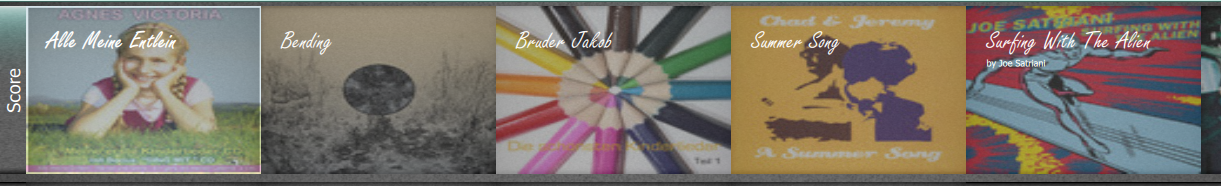
\includegraphics[width=\textwidth]{album_covers}

\paragraph{Workflow}
This is an overview of how album art for the individual score files is loaded.
\begin {enumerate}
	\item {A delegate representing a score file is created. At this point meta data of the score have been read from the file header and are requested by the delegate.}
	\item {The delegate calls the function {\tt requestImage} passing its corresponding song title and artists as well as a reference to delegate itself to the function.}	
	\item {The function {\tt requestImage}} calls the function {\tt request} (as explained below) passing the title of the song, the reference to the delegate as well as a callback function defined at this point.
	\item {The function {\tt request} asynchronously executes a HTTP reqeust to the iTunes API. The callback function that was defined in the last step will be called once the HTTP request is completed. The reference to the delegate and the content of the HTTP response will be passed to the callback function. }
	\item {The callback function parses the response and extracts the URL of the image to be displayed by the delegate.}
	\item {Finally the callback function calls a function of the delegate which will display the image located at the specified URL.}
\end {enumerate}
\paragraph{iTunes API}
The iTunes API supplies meta data on music releases and artists. Comminucation with the API is based on HTTP.
JSON is used for representing the delivered data.
The terms of use allow using promotional contents including song previews and album art for promotional purposes only.
\paragraph{HTTP communication in JavaScript}
The XMLHttpRequest API is used for sending HTTP requests in JavaScript.
The event listener {\tt onreadystatechange} will be invoked on four different occasions. The state of the request is stored in the {\tt readyState} property of the request object.
Only the last state change is of interest to the application. This occurs when the content of the response has finished loading. 
The method {\tt open} initializes the {\tt XMLHttpRequest}-object.
At this point the HTTP request method is specified. The third parameter causes the request to be executed asynchronously.
No data is sent to the server along with this request.
\begin{lstlisting}
    function request(url, del, callback) {
            var xhr = new XMLHttpRequest();
            xhr.onreadystatechange = (function(myxhr) {

                return function() {
                    // finished
                    if (xhr.readyState === 4) {
                        callback(myxhr, del);
                    }
                }

            })(xhr);
            xhr.open('GET', url, true);
            xhr.send('');
    }
\end{lstlisting}
\paragraph{Parsing JSON in JavaScript}
JSON is an open data format primarily intended for exchanging data between applications. JSON is a proper subset of JavaScript. For this reason parsing JSON in JavaScript turns out to be particularly neat.
\begin{lstlisting}
	// translate response into object
	var receivedData = eval('new Object(' + o.responseText + ')');
	
	// access elements inside json object with dot notation
	if (receivedData.results !== undefined) {
	    if (receivedData.results[0].artworkUrl100 !== undefined) {
	        var uri = receivedData.results[0].artworkUrl100
	        delegate.setImage(uri)
	    }
	}
\end{lstlisting}
The function {\tt eval()} evaluates or executes the supplied JavaScript code. In the listing above the function returns a new object containing the JSON-notated data coming rom the HTTP response. \\ Based on the structure of the JSON content accessing the data is straightforward.
\chapter[In-Game User Interface Implementation \textsuperscript{Novotny}]{In-Game User Interface Implementation}
\label{chap:In-Game User Interface}

\section{Organization of this Chapter}
This chapter treats the implementation of the in-game user interface. A section has been devoted to each of three display options the application provides:

\begin {itemize}
	\item {Piano Roll}
	\item {Score View}
	\item {Tablature View}
\end {itemize}

The first section gives an overview of the architechture behind the in-game user interface.

\section{Design}
The implementation of all three display options is based on the {\tt QQuickItem} drawing approach explained in the \textit{Technologies} chapter (\ref{chap:Technologies}). 

The three display options require many common resources. Application logic and calculations used in for the individual display options are very similar in a number of ways. The class hierachy used for implementing the display options helps avoid redundancies while maintaining flexibility.

\subsection{Visuals}
{\tt Visuals} handles tasks relevant to all display options. These tasks are described throughout the following subsections.

\subsubsection{Providing Data}
{\tt Visuals} provides a property {\tt game} of type {\tt MainGame}.
This property is used for accessing:
\begin {itemize}
	\item {tracks of the score}
	\item {track played by the user}
\end {itemize}

\subsubsection{Scrolling}
\subsubsection{Determining the appropriate Time Span to display}
In order to provide relevant instructions and feedback to the user, the amount of information presented needs to be adjusted to the complexity of the score. Primarily this means displaying the right amount of notes simultaneously.
{\tt Visuals} provides the attribute {\tt msPerScreen} which sets the time span to be displayed on the screen. This attribute is set to an appropriate value depending on the density of notes in the track. A value of 1000 means that one second of music will be displayed. 


\subsection{QQI\_Based\_Visuals}
The class {\tt QQI\_Based\_Visuals} extends {\tt Visuals}. This class offers a range of functions relevant for drawing using the {\tt QtQuickItem} based approach.
The reason for introducing this second subclass is maintaining flexibility in terms of how the components are painted. While experience has shown that using the canvas-based drawing approach is not suitable for drawing complex real-time oriented components due to limitations of the current rendering implementation this architecture allows quick adoptions in the future.
Functions provided by {\tt QQI\_Based\_Visuals} are discussed throughout the following subsections.

\subsubsection{Converting Time Stamps to Positions}
Objects such as:
\begin{itemize}
	\item{notes}
	\item{bar lines}
	\item{bending profiles}
\end{itemize}
are a associated with a timestamp relative to the start of the song.
The function {\tt calculatePosition} has a number of overloads. It accepts either a time stamp or a {\tt Note} object and a boolean flag indicating whether or not the object is contained in the score (as opposed to played by the user). {\tt calculatePosition} returns the horizontal position of objects taking the following factors into account:
\begin{itemize}
	\item{scaling of the component}
	\item{horizontal shifts that occur if the song is started at a position other than its beginning (refer to the chapter on \textit{Design} for further details)}
\end{itemize}

\subsubsection{Loading Textures}
Textures such as:
\begin{itemize}
	\item{triangle textures (pointing left and right) that indicate timing mistakes}
	\item{digit textures required for printing the score above notes}
\end{itemize}
are required by all display options. The function {\tt loadTextures} loads these textures.
Note that every display option implements their on {\tt loadTextures} function which calls the {\tt QQI\_Based\_Visuals::loadTextures} and loads add loads additionals textures it requires.

\subsubsection{Drawing Bar Lines}
Drawing bar lines significantly increases the readability of scores and is used every display option.
{\tt QQI\_Based\_Visuals} offers the function {\tt getBarsNode}. The function returns a {\tt QSGNode} containing at least all bar nodes in the visible scope. This node can be added to the parent node by the calling display option.

The start time of every bar is contained in the {\tt Score} object maintained by the {\tt game} object. {\tt getBarsNode} uses the function {\tt calculatePosition} to position the bar lines accordingly.

\subsubsection{Displaying Target Notes and Played Notes}
The function {\tt getTargetNotes} returns a node containing all target notes of the selected track. 
Similarly the function {\tt getPlayedNotes} returns a node containing all notes played by the user.

In order to improve performance only notes within the visible time range are added to the node.
The variable {\tt startIndex} stores the index of the first note within the track that needs to be drawn. This variable is updated continuously.

The functions use the virtual function {\tt getNodeForNote} that is implemented by every display option. This allows the display option to define the appearance of the notes while avoiding redundancies.

\subsubsection{Score for Target Notes}
As explained in \textit{User Interaction Concept} (\ref{chap:UserInteractionConcept}) every note of the track the user is trying to play is associated with a numeric score. The maximum score for every note is 50 points, deductions are made for playing the wrong pitch and timing mistakes.

By default every target note has a score of -1. This value is updated by the {\tt Evaluator} as soon as a played note is associated with the target note. If one of the display options recognizes a target note with a non-negative score the numeric value is printed above the target note.

The function {\tt getNumberNode(int number, int size, int left, int top)} returns a {\tt QSGNode} that displays the specified number and has the specified position and size.

\subsubsection{Drawing Text Nodes}
Qt does not offer a mechanism for drawing text nodes. Drawing numeric values representing the score of a note requires a number of steps. 

The funtion {\tt loadTextures} creates a {\tt QList} of textures containing a texture for every digit between 0 and 9.
This is done by loading an image containing all digits and splitting the image into ten equally sized pieces using the function {\tt createSubImage}.

\begin{lstlisting}
	QImage QQI_Based_Visuals::createSubImage(QImage* image, const QRect & rect)
	{
	    size_t offset = rect.x() * image->depth() / 8
	                    + rect.y() * image->bytesPerLine();
	    return QImage(image->bits() + offset, rect.width(), rect.height(),
	                  image->bytesPerLine(), image->format());
	}
\end{lstlisting}

The function {\tt getNumberNode} creates the node using the following steps:

\begin{enumerate}
	\item{split the number into a list of digits}
	\item{create a parent node that will contain all digit nodes}
	\item{create a {\tt QSGSimpleTextureNode} for every digit using the textures created in {\tt loadTextures} and add it to the parent node}
\end{enumerate}

\subsection{Drawing notes in the score view}
Drawing notes in the score view is special because the {\tt QSGTexture}s are 
generated from Scalable Vector Graphic (SVG) files. SVG files are a form of picture format where, instead of saving an array of pixels in the file, the drawing is described in XML in the form of shapes, colors or gradients. To generate a texture from an SVG file several steps have to be made. The following sample code shows a simple way to generate textures.
\begin{lstlisting}
 QSvgRenderer svgRenderer(texturePath);
 QImage image(width, height, QImage::Format_ARGB32);
 image.fill(0xFFFFFF);
 QPainter painter(&image);
 painter.setRenderHint(QPainter::Antialiasing);
 svgRenderer.render(&painter);
 QSGTexture *texture = window()->createTextureFromImage(image);
\end{lstlisting}

The {\tt QImage} object is the temporary object that will store a rendered version of the SVG file. {QSvgRenderer} uses the provided {\tt QPainter} to paint the SVG document into the {\tt QImage}. After that {\tt createTextureFromImage()} can be used to generate a texture from the QImage for use in the scene graph.
\\
This type of texture is used for the following types of objects:
\begin{enumerate}
\item note textures in black, green and red
\item dotted notes
\item sharp (\#) sign
\item grace notes
\item clef
\end{enumerate}

\subsection{Painting Process for all Display Options}
Ever display options implements the function {\tt updatePaintNode} defined in {\tt QQuickItem}. The drawing process implemented in these functions generally follows the following flow:
\begin{enumerate}
	\item{
		Preparations such as:
		\begin{itemize}
			\item{deleting all contents of the scene graph and creating a new parent node (refer to the chapter \textit{Technologies} (\ref{chap:Technologies}))}
 			\item{retrieving the current game time}
			\item{updating the scroll bar position}
		\end{itemize}
		Where possible these preparations are done by functions of {\tt QQI\_Based\_Visuals} in a generic way in order to avoid code duplicates.
	}
	\item{
		Drawing objects specific to the display option such as:
		\begin{itemize}
			\item{a piano graphic and coloured lines in {\tt PianoRoll}}
			\item{strings in {\tt TablatureView}}
			\item{clef in {\tt ScoreView}}
		\end{itemize}
	}
	\item{
		Drawing objects required by all display options such as:
		\begin{itemize}
			\item{a vertical line indicating the current point in time}
			\item{bar lines}
		\end{itemize}
		The correpsonding nodes for these objects are created by {\tt QQI\_Based\_Visuals}.
	}
	\item{
		Drawing target notes and played notes. This process has been covered in the previous section.
	}
\end{enumerate}

\include{ideenfuerdiezukunft}


%%%----------------------------------------------------------

%\printindex

%\printglossaries

%Literaturverzeichnis
\clearpage
\addcontentsline{toc}{chapter}{\bibname}

\bibliographystyle{bababbrv} 
%options: babplain, babunsrt, bababbrv, babalpha 
%         babplain-fl etc: first/lastname 
%         babplain-lf etc: last/firstname
\bibliography{literatur}     %BibTeX-Datei literatur.bib


\chapter{Conclusion}

\section{Idea and Motivation}

We got the idea when we were talking about pattern recognition in audio signals. Novotny being a hobbyist bassist in the band \emph{Das Nusswerk} always wanted an application that provided this sort of functionality. 

In May 2013 we started creating prototypes of components in Java. If we had not started back then we probably could not have finished the project in time.

Since we all have a musical background we had a lot of fun developing and testing our program. 

\section{Problems}

In the process of developing this program we faced multiple problems.

\begin{itemize}
	\item Lack of documentation about the Qt framework.
	\item Some MIDI devices do not comply with the General MIDI specification.
	\item Audio queue adds a lot of latency that has to be considered and compensated.
	\item Guitars differ widely in frequency spectrum.
	\item Platform specific bugs.
\end{itemize}

\section{Plans for the Future}



\begin{itemize}
	\item Support for additional instruments.
	\item Support for more display methods.
	\item Support for other platforms like Mac.
\end{itemize}

\section{}
\chapter{Curriculum vitae}

%\pagebreak

\section{Felix Kugler}
I was born on the 18\textsuperscript{th} of August in 1994 in Oberpullendorf. I live with my parents and my younger sister in St. Margarethen in Burgenland, Austria.

My mother, Sylvia Kugler is teacher at the Volksschule Rust. My father is music teacher for guitar at the music school in Eisenstadt.

\subsection{Education}
\begin{description}
	\item[2000 - 2004] Volksschule St. Margarethen
	\item[2004 - 2005] Hauptschule Rust
	\item[2005 - 2009] "Astrid Lindgren Zentrum" in Liesing, Vienna
	\item[2009 - 2014] HTL Wiener Neustadt
\end{description}

\subsection{Work Experience}
\begin{description}
	\item[2012] Burgenländische Landesregierung for one month
	\item[2013] BEWAG Burgendland for one month
\end{description}

\subsection{Leisure}
I took piano lessons for multiple years and I've been playing around with audio processing and pattern recognition before this project.


%\pagebreak

\section{Alfred Neumayer}

I was born on the 2\textsuperscript{nd} of October, 1992 in Wiener Neustadt. I live with my parents in Purbach, a small city near Eisenstadt, Austria.

My mother Heidi used to work as a nurse until she retired while my father, Alfred, is a car mechanic.

\subsection{Education}
\begin{description}
\item[1999 - 2003] Volksschule Purbach am Neusiedlersee
\item[2003 - 2007] Gymnasium der Diözese Eisenstadt
\item[2007 - 2014] HTL Wiener Neustadt
\end{description}

\subsection{Work experience}
\begin{description}
	\item[July and August 2012] Thales GmbH
	\item[July 2013] Thales GmbH
\end{description}
\subsection{Hobbies}
When I'm not spending time with friends and family, or making music, I'm active in the world of open source sofware. I also like working on software for smart phones and tables, especially their technological underpinnings like operating systems.

\pagebreak

\section{Daniel Novotny}
I was born on the 12\textsuperscript{th} of July in 1995 in Pöttsching. 
I live with my parents, Ursula Novotny and Anton Toth, in Pöttsching, Burgenland, Austria.
\subsection{Education}
\begin{description}
	\item[2001 - 2005] Volksschule Pöttsching
	\item[2005 - 2009] Bundesgymnasium und Bundesrealgymnasium Mattersburg
	\item[2009 - 2014] HTL Wiener Neustadt
\end{description}

\subsection{Work Experience}
\begin{description}
	\item[July 2011] Seal Maker Produktions- und Vertriebs GmbH, IT Department
	\item[July 2012] Seal Maker Produktions- und Vertriebs GmbH, IT Department
\end{description}

\subsection{Leisure}
I have been playing guitar and bass guitar for many years which has been the reason for my interest in this project.

\chapter{Acknowledgements}

We want to express our gratitude towards a lot of people that helped us along the way.

A special thank you goes to our advisor Dipl.-Ing. Dr. Günter Kolousek for his support, expertise and his patience.

We would like to thank our parents for their constant support: Sylvia and Albert Kugler, Ursula Novotny and Anton Toth, Heidi and Alfred Neumayer.



%%%----------------------------------------------------------


\end{document}
